%%%%%%%%%%%%%%%%%%%%%%%%%%%%%%%%%%%%%%%%%
% Beamer Presentation
% LaTeX Template
% Version 2.0 (March 8, 2022)
%
% This template originates from:
% https://www.LaTeXTemplates.com
%
% Author:
% Vel (vel@latextemplates.com)
%
% License:
% CC BY-NC-SA 4.0 (https://creativecommons.org/licenses/by-nc-sa/4.0/)
%
%%%%%%%%%%%%%%%%%%%%%%%%%%%%%%%%%%%%%%%%%

%----------------------------------------------------------------------------------------
%	PACKAGES AND OTHER DOCUMENT CONFIGURATIONS
%----------------------------------------------------------------------------------------

\documentclass[
	11pt, % Set the default font size, options include: 8pt, 9pt, 10pt, 11pt, 12pt, 14pt, 17pt, 20pt
	% t, % Uncomment to vertically align all slide content to the top of the slide, rather than the default centered
	%aspectratio=169, % Uncomment to set the aspect ratio to a 16:9 ratio which matches the aspect ratio of 1080p and 4K screens and projectors
]{beamer}

\usepackage{xmpmulti}
\usepackage{varwidth}
\usepackage[]{mdframed}
\usepackage{graphicx}
\usepackage{booktabs}
\usepackage{caption}

\usepackage{listings}
\usepackage{color}

\usepackage{algpseudocode}

\graphicspath{{Images/}{./}} % Specifies where to look for included images (trailing slash required)

\usepackage{booktabs} % Allows the use of \toprule, |rule and \bottomrule for better rules in tables
% \usepackage[dvipsnames]{xcolor}

%----------------------------------------------------------------------------------------
%	SELECT LAYOUT THEME
%----------------------------------------------------------------------------------------

% Beamer comes with a number of default layout themes which change the colors and layouts of slides. Below is a list of all themes available, uncomment each in turn to see what they look like.

% \usetheme{default}
% \usetheme{AnnArbor}
% \usetheme{Antibes}
% \usetheme{Bergen}
% \usetheme{Berkeley}
\usetheme{Berlin} % *
%\usetheme{Boadilla}
%\usetheme{CambridgeUS}
%\usetheme{Copenhagen}
%\usetheme{Darmstadt}
%\usetheme{Dresden}
%\usetheme{Frankfurt}
%\usetheme{Goettingen}
%\usetheme{Hannover}
%\usetheme{Ilmenau}
%\usetheme{JuanLesPins}
%\usetheme{Luebeck}
% \usetheme{Madrid} % *
%\usetheme{Malmoe}
%\usetheme{Marburg}
%\usetheme{Montpellier}
%\usetheme{PaloAlto}
%\usetheme{Pittsburgh}
%\usetheme{Rochester}
%\usetheme{Singapore}
% \usetheme{Szeged}
% \usetheme{Warsaw}

%----------------------------------------------------------------------------------------
%	SELECT COLOR THEME
%----------------------------------------------------------------------------------------

% Beamer comes with a number of color themes that can be applied to any layout theme to change its colors. Uncomment each of these in turn to see how they change the colors of your selected layout theme.

% \usecolortheme{albatross}
\usecolortheme{beaver}
% \usecolortheme{beetle}
% \usecolortheme{crane}
% \usecolortheme{dolphin}
% \usecolortheme{dove}
% \usecolortheme{fly}
% \usecolortheme{lily}
% \usecolortheme{monarca}
% \usecolortheme{seagull}
% \usecolortheme{seahorse}
% \usecolortheme{spruce}
% \usecolortheme{whale}
% \usecolortheme{wolverine}

%----------------------------------------------------------------------------------------
%	SELECT FONT THEME & FONTS
%----------------------------------------------------------------------------------------

% Beamer comes with several font themes to easily change the fonts used in various parts of the presentation. Review the comments beside each one to decide if you would like to use it. Note that additional options can be specified for several of these font themes, consult the beamer documentation for more information.

\usefonttheme{default} % Typeset using the default sans serif font
% \usefonttheme{serif} % Typeset using the default serif font (make sure a sans font isn't being set as the default font if you use this option!)
% \usefonttheme{structurebold} % Typeset important structure text (titles, headlines, footlines, sidebar, etc) in bold
% \usefonttheme{structureitalicserif} % Typeset important structure text (titles, headlines, footlines, sidebar, etc) in italic serif
% \usefonttheme{structuresmallcapsserif} % Typeset important structure text (titles, headlines, footlines, sidebar, etc) in small caps serif

%------------------------------------------------

% \usepackage{mathptmx} % Use the Times font for serif text
\usepackage{palatino} % Use the Palatino font for serif text

% \usepackage{helvet} % Use the Helvetica font for sans serif text
% \usepackage[default]{opensans} % Use the Open Sans font for sans serif text
% \usepackage[default]{FiraSans} % Use the Fira Sans font for sans serif text
\usepackage[default]{lato} % Use the Lato font for sans serif text

%----------------------------------------------------------------------------------------
%	SELECT INNER THEME
%----------------------------------------------------------------------------------------

% Inner themes change the styling of internal slide elements, for example: bullet points, blocks, bibliography entries, title pages, theorems, etc. Uncomment each theme in turn to see what changes it makes to your presentation.

\useinnertheme{default}
% \useinnertheme{circles}
% \useinnertheme{rectangles}
%\useinnertheme{rounded}
% \useinnertheme{inmargin}

%----------------------------------------------------------------------------------------
%	SELECT OUTER THEME
%----------------------------------------------------------------------------------------

% Outer themes change the overall layout of slides, such as: header and footer lines, sidebars and slide titles. Uncomment each theme in turn to see what changes it makes to your presentation.

%\useoutertheme{default}
\useoutertheme{infolines}
% \useoutertheme{miniframes}
% \useoutertheme{smoothbars}
% \useoutertheme{sidebar}
% \useoutertheme{split}
% \useoutertheme{shadow}
% \useoutertheme{tree}
% \useoutertheme{smoothtree}

\usepackage{unicode-math}
\setmathfont{Libertinus Math} % **

%\setbeamertemplate{footline} % Uncomment this line to remove the footer line in all slides
\setbeamertemplate{footline}[page number] % Uncomment this line to replace the footer line in all slides with a simple slide count

\setbeamertemplate{navigation symbols}{} % Uncomment this line to remove the navigation symbols from the bottom of all slides

\definecolor{green}{HTML}{00BB50}
\definecolor{red}{HTML}{FE0000}
\definecolor{yellow}{HTML}{FFCC00}
% \definecolor{crimson}{RGB}{220,20,60}
\definecolor{crimson}{HTML}{A30000}
\definecolor{bbg}{HTML}{D9D9D9}

\setbeamercolor{block body}{bg = bbg, fg = black}
\setbeamercolor{block title}{bg = gray!120, fg= white}
\setbeamercolor{palette secondary}{bg = gray!135, fg = white}

\setbeamercolor{item}{fg=crimson} % Set bullet points to crimson (RGB: 204, 0, 102)
\setbeamercolor{enumerate item}{fg=crimson} % Set enumerated items to crimson (RGB: 204, 0, 102)

\setbeamercolor{block title example}{bg = gray!120, fg = white}
\setbeamercolor{block body example}{bg = bbg, fg = black}

\setbeamercolor{structure}{bg=red}

%----------------------------------------------------------------------------------------
%	PRESENTATION INFORMATION
%----------------------------------------------------------------------------------------

\title[Blockchain]{Borůvka's Algorithm \\ The Oldest MST Algorithm We Know} % The short title in the optional parameter appears at the bottom of every slide, the full title in the main parameter is only on the title page

% \subtitle{Optional Subtitle} % Presentation subtitle, remove this command if a subtitle isn't required

\author[]{ Presented by \\ Ali Tavassoly \\ \vspace*{0.5cm} Course conducted by \\ DR. Alireza Zarei} % Presenter name(s), the optional parameter can contain a shortened version to appear on the bottom of every slide, while the main parameter will appear on the title slide

\institute[]{Sharif University of Technology } % Your institution, the optional parameter can be used for the institution shorthand and will appear on the bottom of every slide after author names, while the required parameter is used on the title slide and can include your email address or additional information on separate lines

\date[]{ Presentation for Advanced Topics in Algorithm} % Presentation date or conference/meeting name, the optional parameter can contain a shortened version to appear on the bottom of every slide, while the required parameter value is output to the title slide

\newcommand{\code}[1]{\colorbox{lightgray}{\lr{#1}}}
\newcommand{\Argmin}[1]{\underset{#1}{\text{argmin}} \hspace{2mm}}

\newcommand{\prob}[2][ ]{\mathbb{P}_{#1}\left[#2\right]}
\newcommand{\expec}[2][ ]{\mathbb{E}_{#1}\left[#2\right]}

%----------------------------------------------------------------------------------------

\begin{document}

%----------------------------------------------------------------------------------------
%	TITLE SLIDE
%----------------------------------------------------------------------------------------

\begin{frame}
	\titlepage % Output the title slide, automatically created using the text entered in the PRESENTATION INFORMATION block above
\end{frame}

%----------------------------------------------------------------------------------------
%	TABLE OF CONTENTS SLIDE
%----------------------------------------------------------------------------------------

% The table of contents outputs the sections and subsections that appear in your presentation, specified with the standard \section and \subsection commands. You may either display all sections and subsections on one slide with \tableofcontents, or display each section at a time on subsequent slides with \tableofcontents[pausesections]. The latter is useful if you want to step through each section and mention what you will discuss.

\begin{frame}
	\frametitle{Presentation Overview} % Slide title, remove this command for no title
	
	\tableofcontents % Output the table of contents (all sections on one slide)
\end{frame}

\section{History}
\begin{frame}
    \tableofcontentscurrent
\end{frame}

\begin{frame}
    \frametitle{History}
    This algorithm first published in 1926 by Otakar Borůvka as 
    a method of constructing an efficient electricity 
    network for Moravia.

    The algorithm was rediscovered by Choquet in 1938;
    again by Florek, Lukasiewicz, Perkal, Steinhaus, 
    and Zubrzycki in 1951; and again by Georges Sollin 
    in 1965.

    This algorithm is frequently called Sollin's algorithm, 
    especially in the parallel computing literature.
\end{frame}


\section{MST Problem}
\begin{frame}
    \tableofcontentscurrent
\end{frame}


\begin{frame}
    \frametitle{Definition of MST problem}
    
    \begin{definition}
        An edge-weighted graph is a graph where we 
        associate weights or costs with each edge.
    \end{definition}

    \begin{definition}
        A minimum spanning tree (MST) of an edge-weighted 
        graph is a spanning tree whose weight 
        (the sum of the weights of its edges) is no 
        larger than the weight of any other spanning tree.
    \end{definition}
\end{frame}

\begin{frame}
    \frametitle{Example of MST}
    \begin{center}
        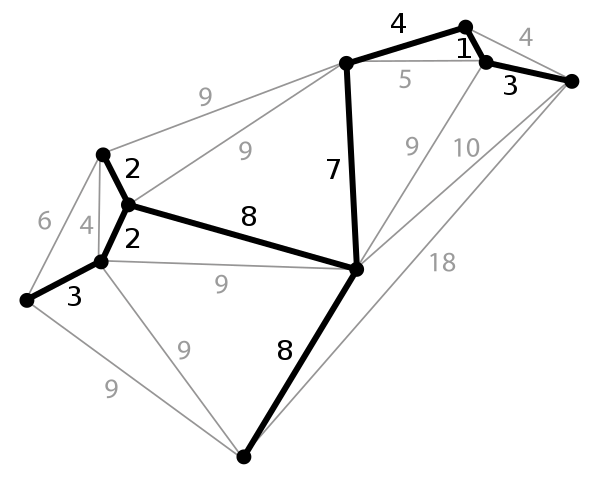
\includegraphics[width = 0.8\textwidth]{images/mst.svg.png}
    \end{center}
\end{frame}

\section{Algorithm}
\begin{frame}
    \tableofcontentscurrent
\end{frame}

\begin{frame}{Algorithm Explanation}
    \begin{beamerboxesrounded}[shadow=true]{Initial state}
        Consider $n$ connected components (each vertex is in its component). So at the initial step, we have chosen no edges and we have $n$ trees.
    \end{beamerboxesrounded}

    \vspace*{0.6cm}    
    \begin{beamerboxesrounded}[shadow=true]{Procedure}
        At each step, there are some trees in the graph.
        For each tree, find the minimum weight of an edge connecting this tree to another one.
        After finding the edges for all the trees, pick them all for our final tree. 
    \end{beamerboxesrounded}

    \vspace*{0.6cm}
    \begin{beamerboxesrounded}[shadow=true]{Final state}
        A tree consisting of $n - 1$ edges having minimum total weight among all possible trees.
    \end{beamerboxesrounded}
\end{frame}

\begin{frame}{Overview}
    \begin{beamerboxesrounded}[shadow=true]{Note}
        Some edges may be chosen for two trees at the same time. We will obviously pick it only once.
    \end{beamerboxesrounded}

    \vspace*{0.5cm}

    \begin{beamerboxesrounded}[shadow=true]{Intuition}
        At each step, we are merging two trees, so we will end up with a tree after some steps.
        \\
        Also, note that we never create a cycle, which is key to the algorithm's effectiveness.
    \end{beamerboxesrounded}
\end{frame}

\begin{frame}
    Here is an example of how the algorithm works:
    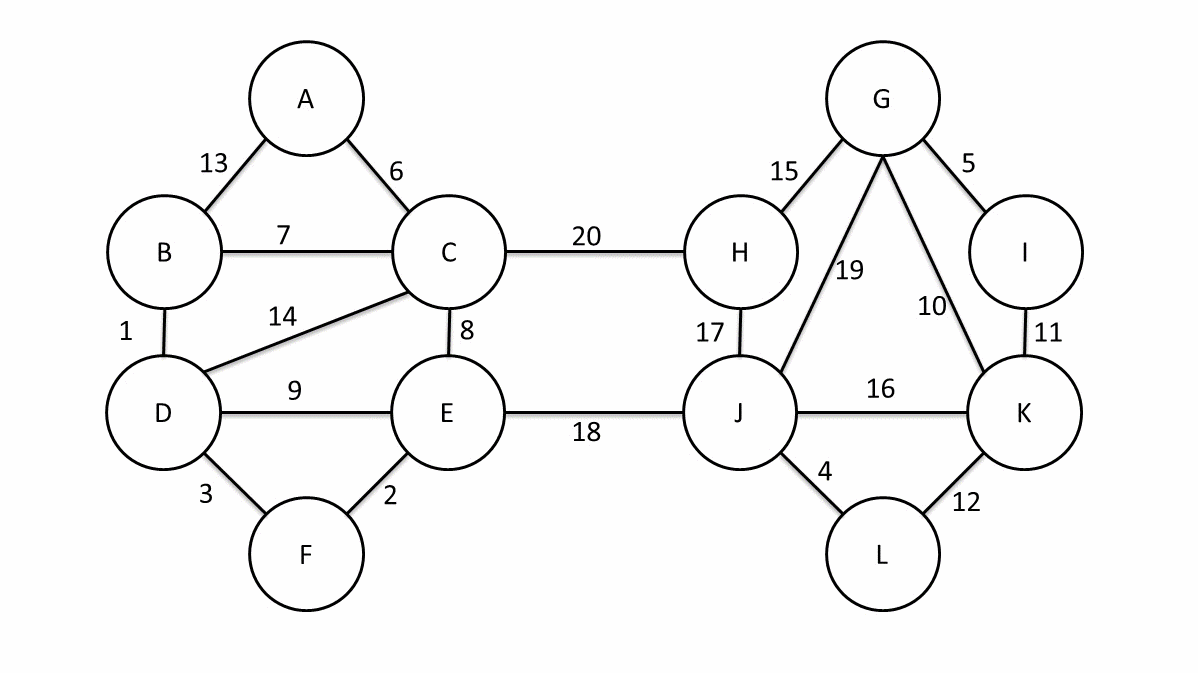
\includegraphics[width = 1\textwidth]{baruvka-example/frame_00_delay-1s.png}
\end{frame}
\begin{frame}
    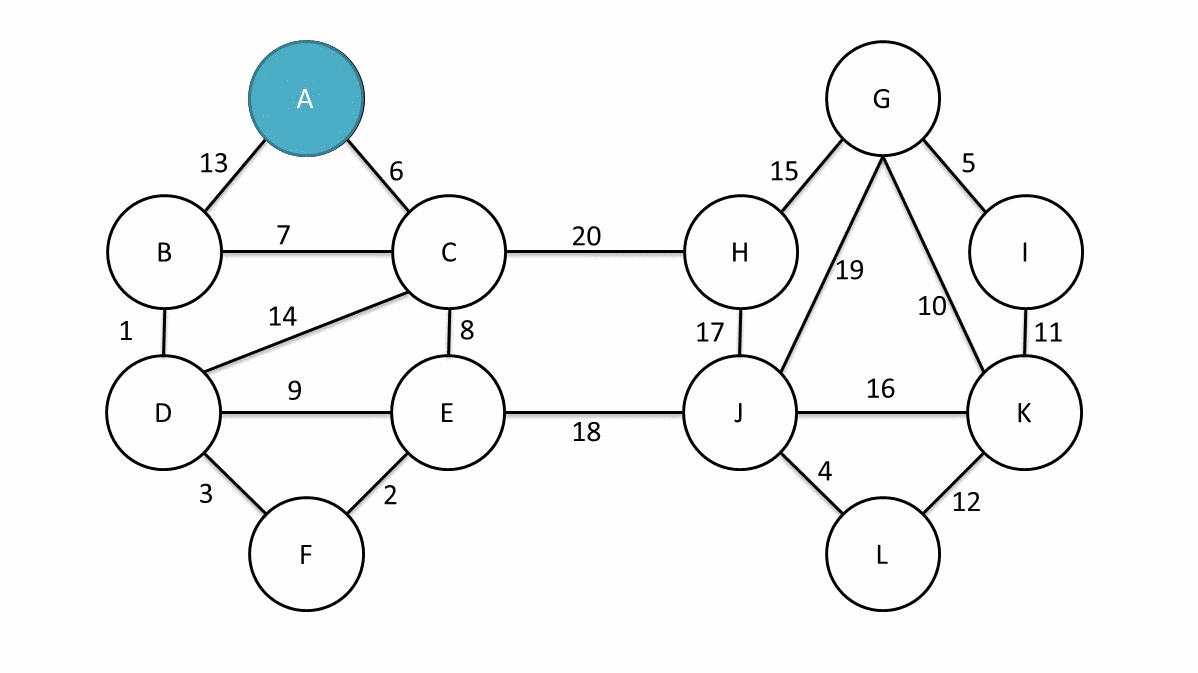
\includegraphics[width = 1\textwidth]{baruvka-example/frame_01_delay-1s.png}
\end{frame}
\begin{frame}
    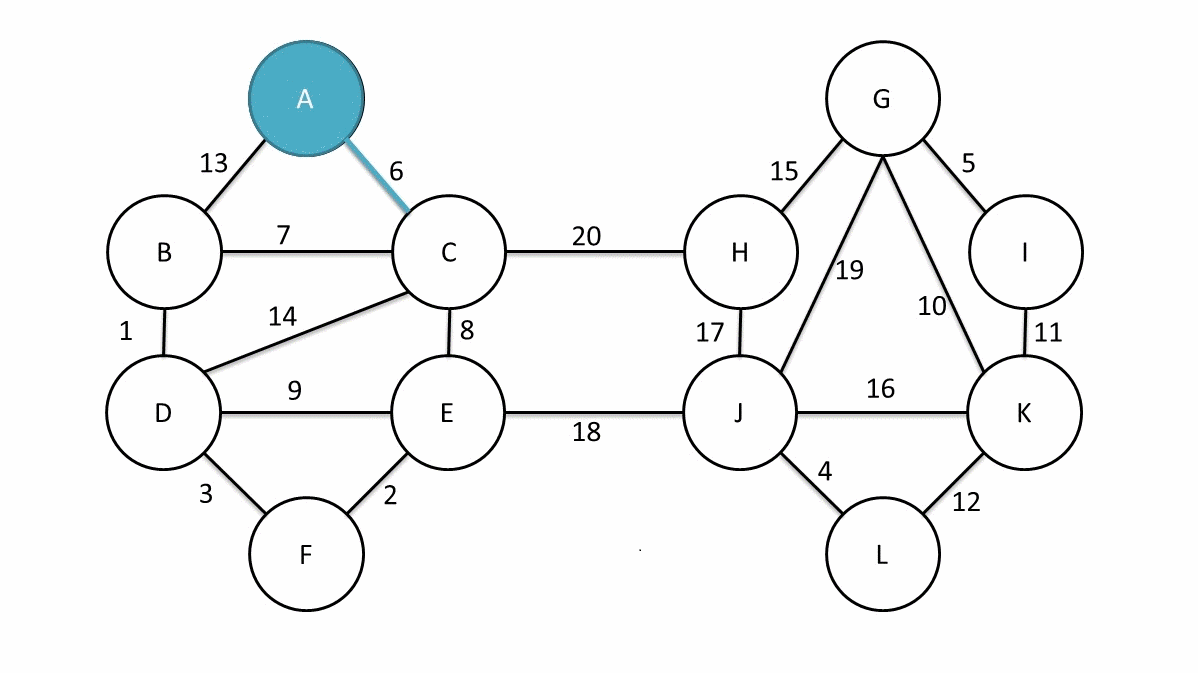
\includegraphics[width = 1\textwidth]{baruvka-example/frame_02_delay-1s.png}
\end{frame}
\begin{frame}
    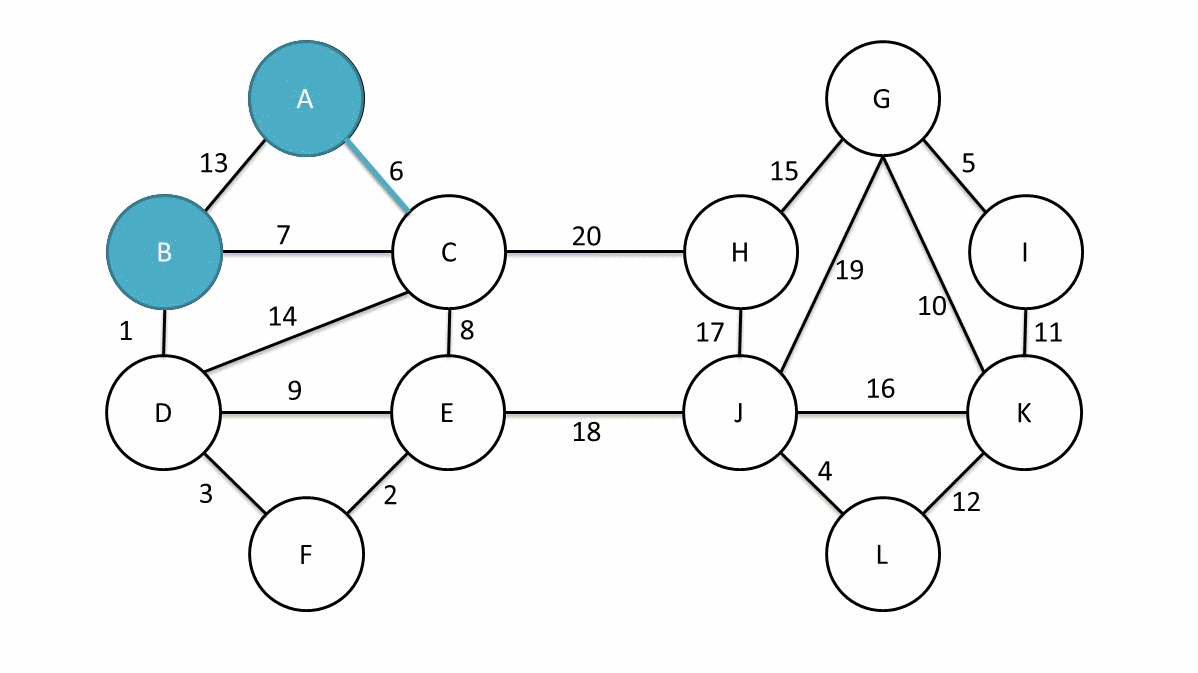
\includegraphics[width = 1\textwidth]{baruvka-example/frame_03_delay-1s.png}
\end{frame}
\begin{frame}
    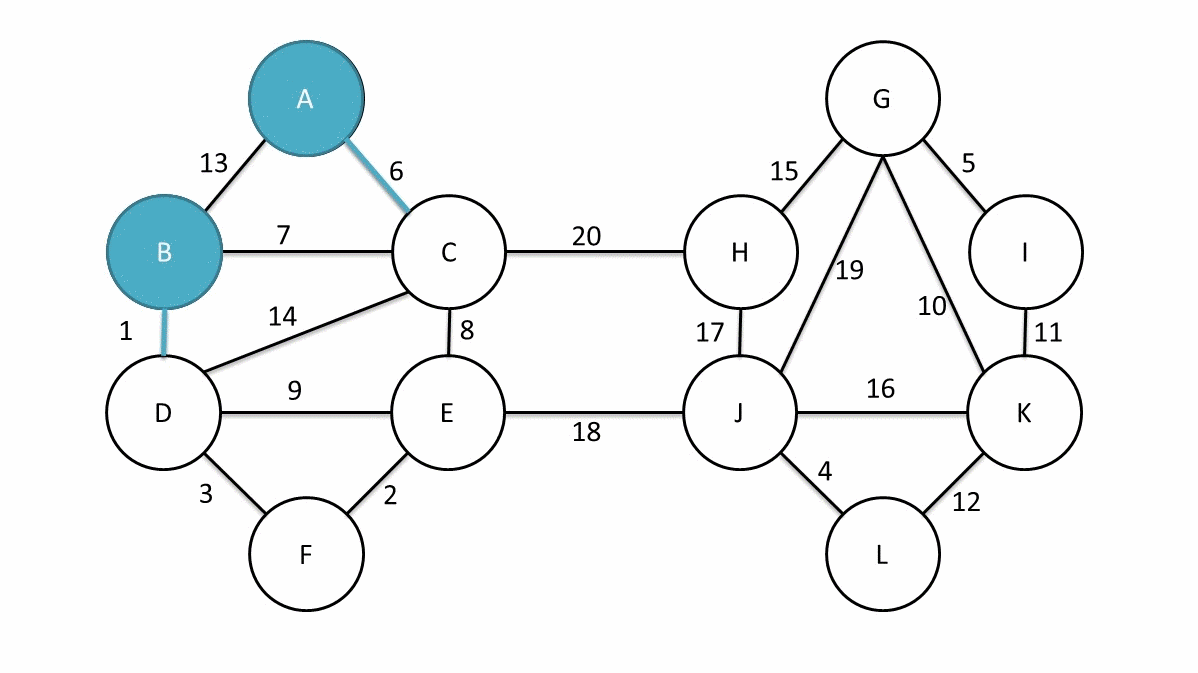
\includegraphics[width = 1\textwidth]{baruvka-example/frame_04_delay-1s.png}
\end{frame}
\begin{frame}
    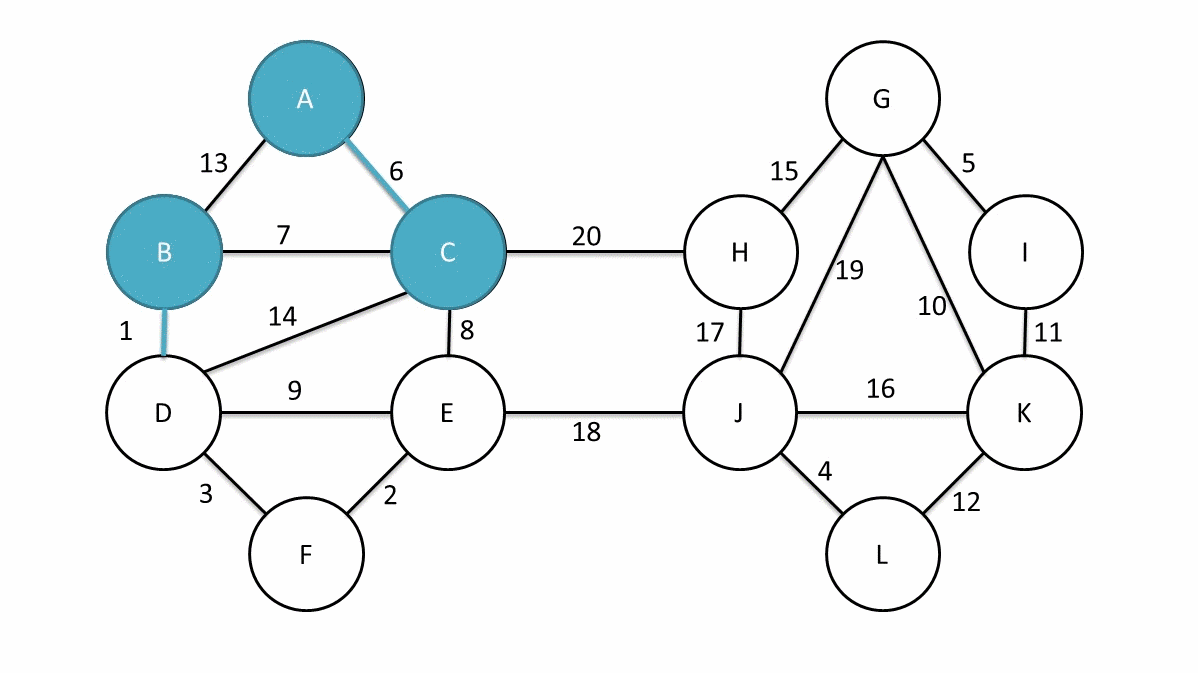
\includegraphics[width = 1\textwidth]{baruvka-example/frame_05_delay-2s.png}
\end{frame}
\begin{frame}
    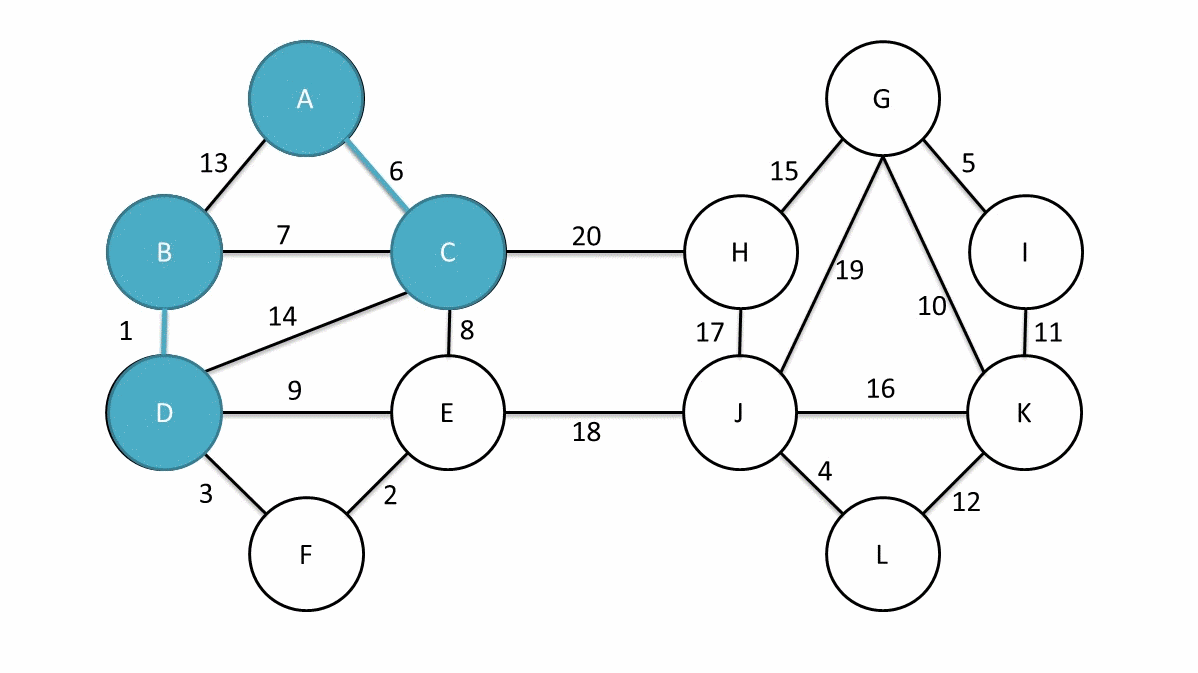
\includegraphics[width = 1\textwidth]{baruvka-example/frame_06_delay-2s.png}
\end{frame}
\begin{frame}
    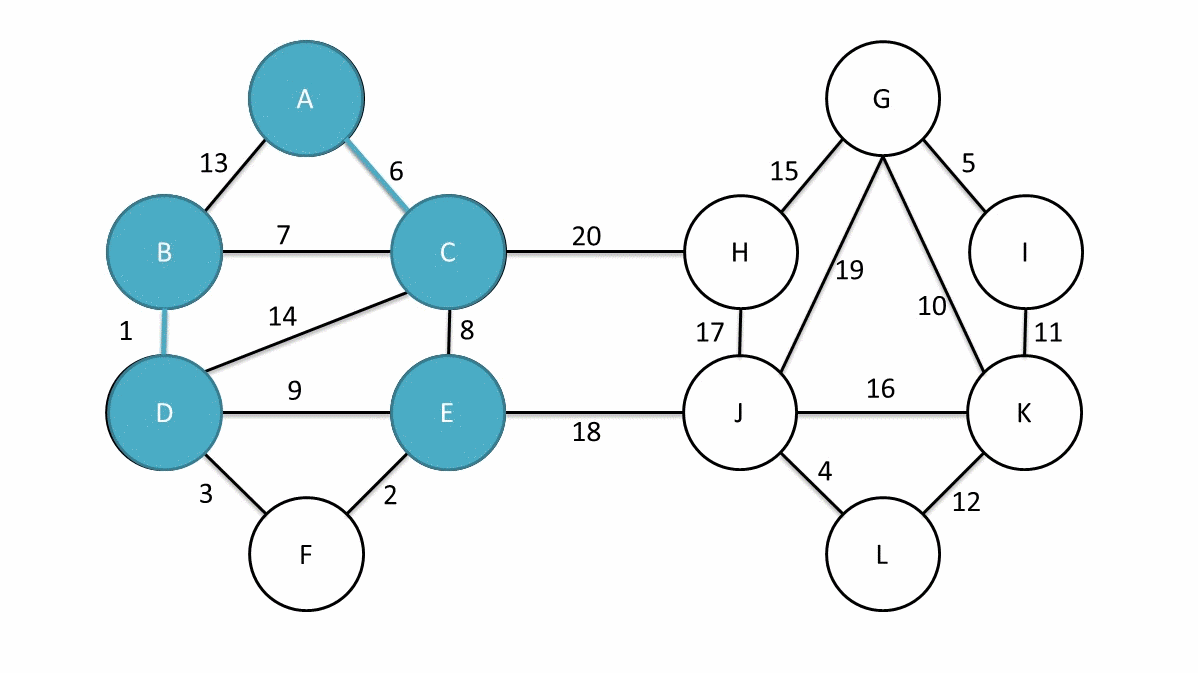
\includegraphics[width = 1\textwidth]{baruvka-example/frame_07_delay-1s.png}
\end{frame}
\begin{frame}
    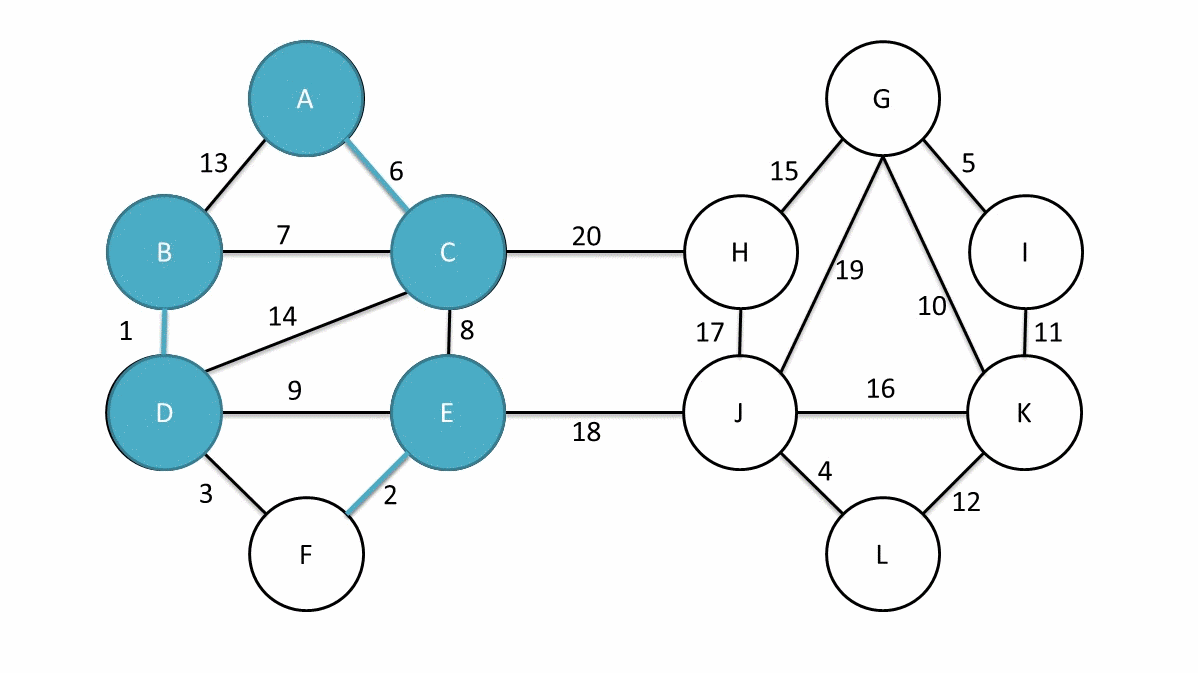
\includegraphics[width = 1\textwidth]{baruvka-example/frame_08_delay-1s.png}
\end{frame}
\begin{frame}
    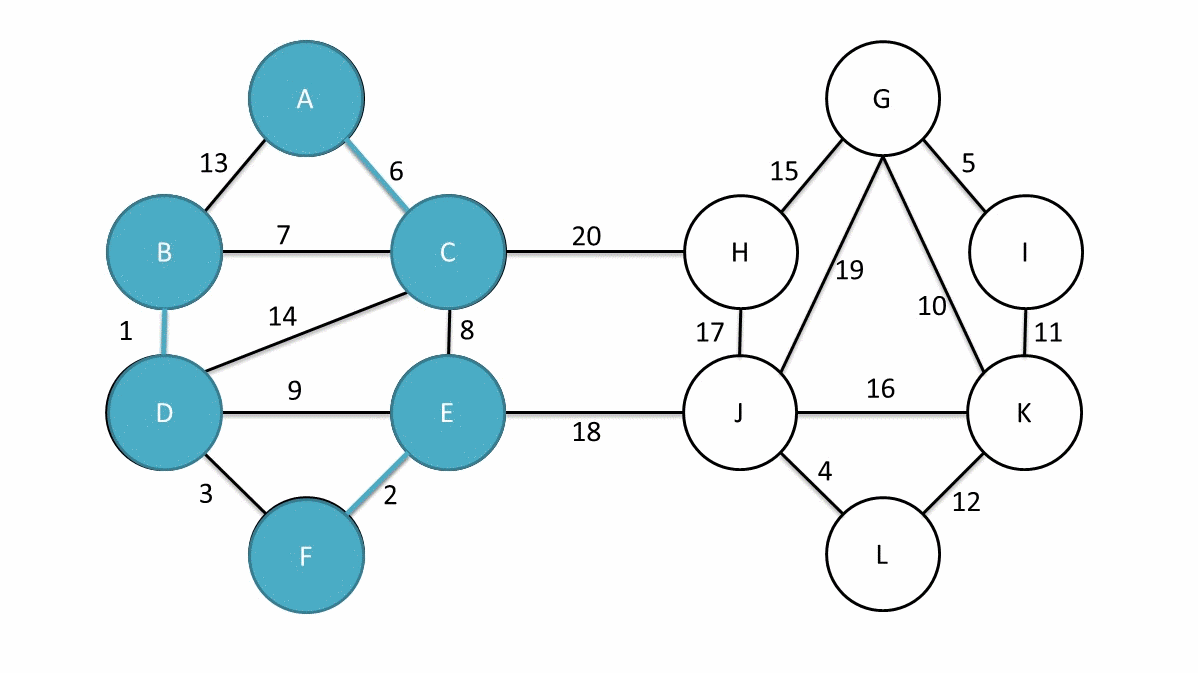
\includegraphics[width = 1\textwidth]{baruvka-example/frame_09_delay-2s.png}
\end{frame}
\begin{frame}
    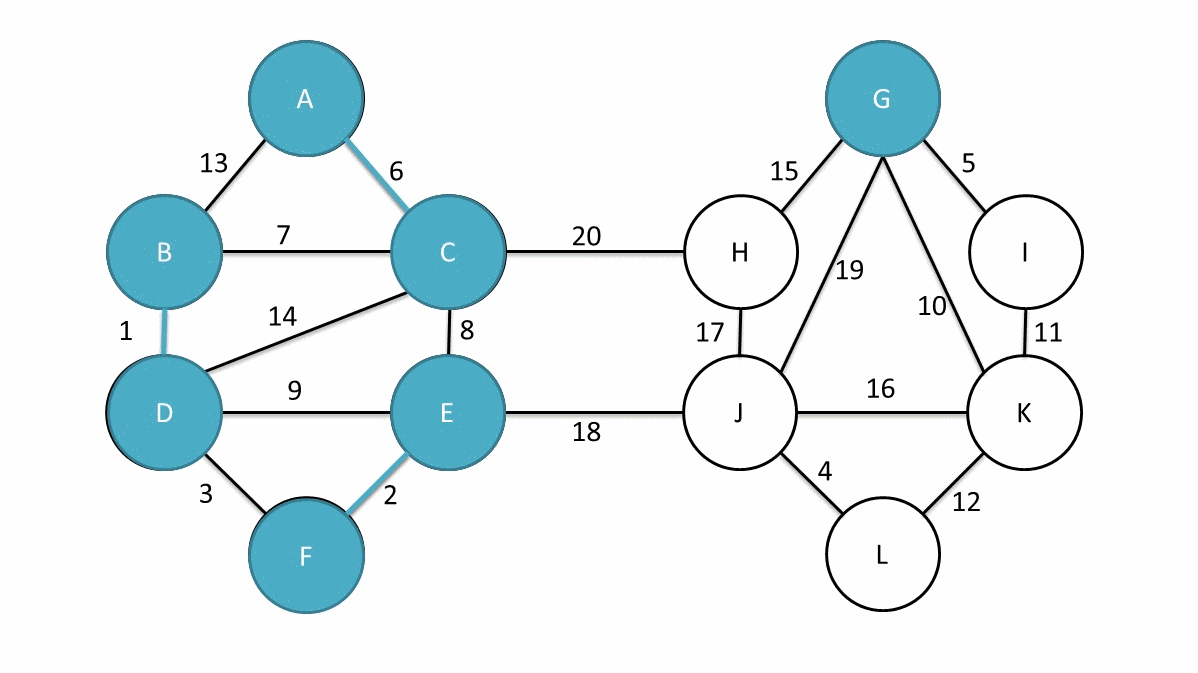
\includegraphics[width = 1\textwidth]{baruvka-example/frame_10_delay-1s.png}
\end{frame}
\begin{frame}
    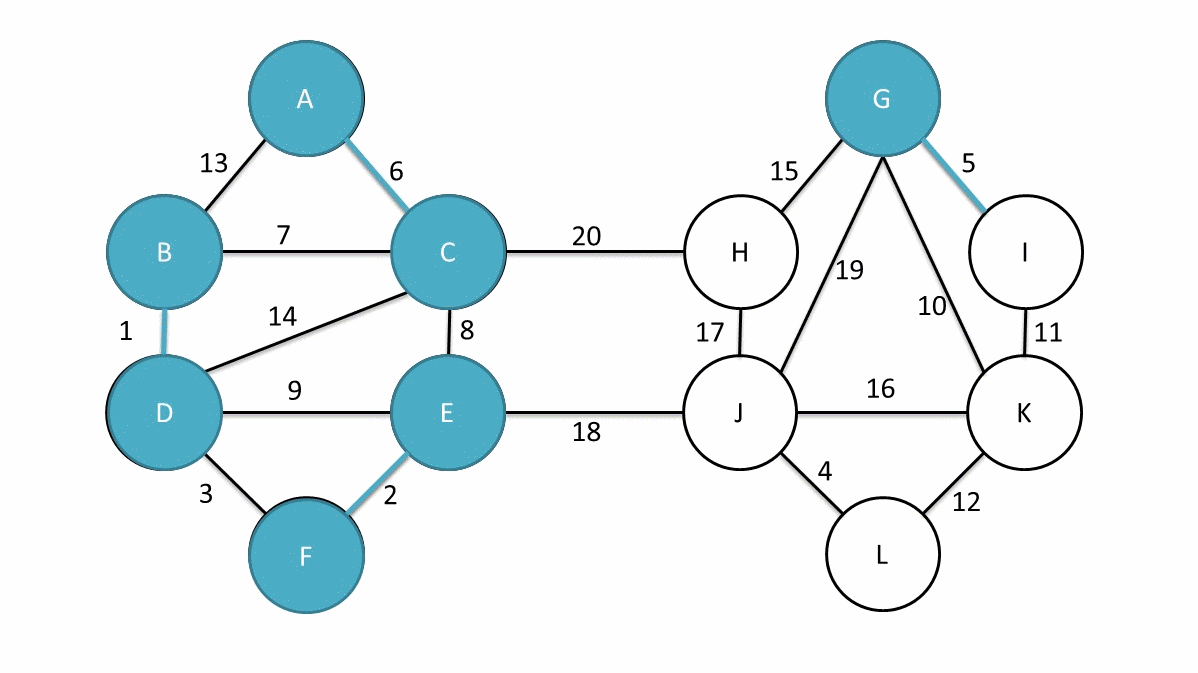
\includegraphics[width = 1\textwidth]{baruvka-example/frame_11_delay-1s.png}
\end{frame}
\begin{frame}
    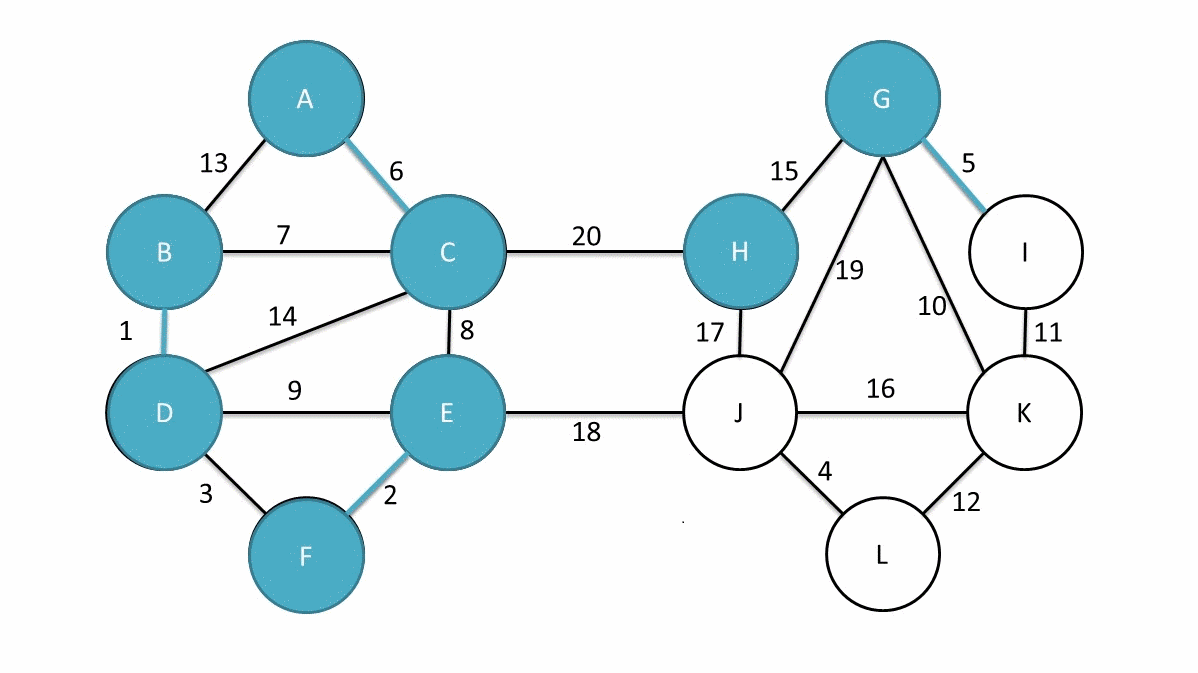
\includegraphics[width = 1\textwidth]{baruvka-example/frame_12_delay-1s.png}
\end{frame}
\begin{frame}
    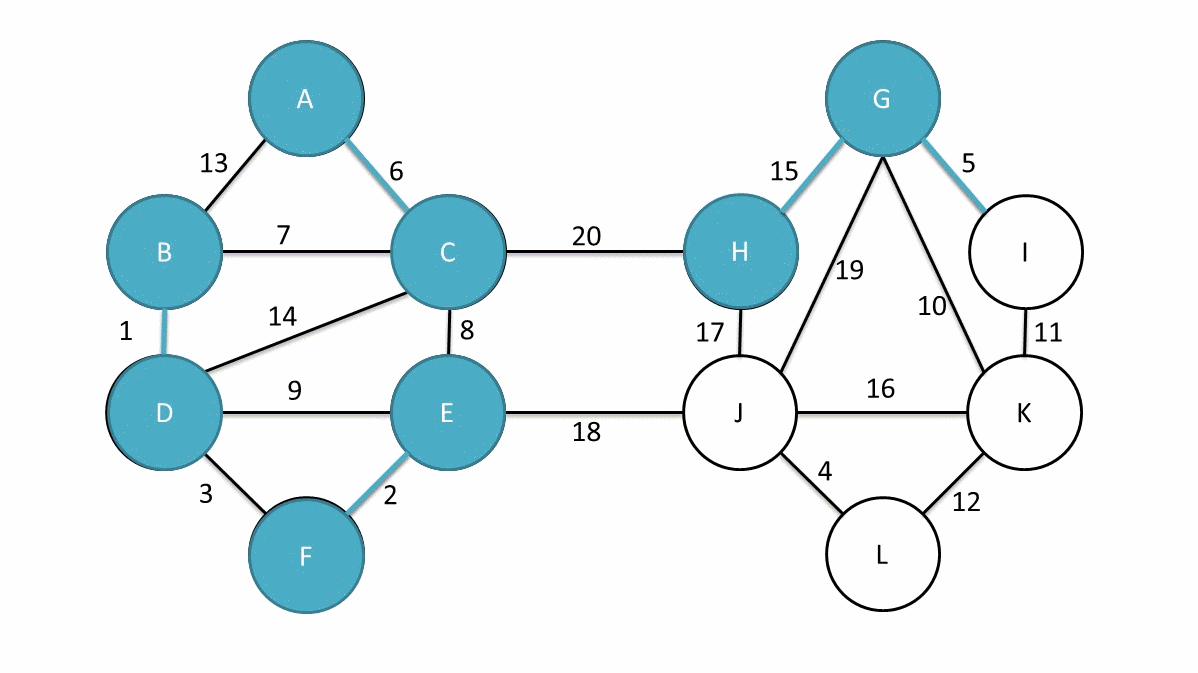
\includegraphics[width = 1\textwidth]{baruvka-example/frame_13_delay-1s.png}
\end{frame}
\begin{frame}
    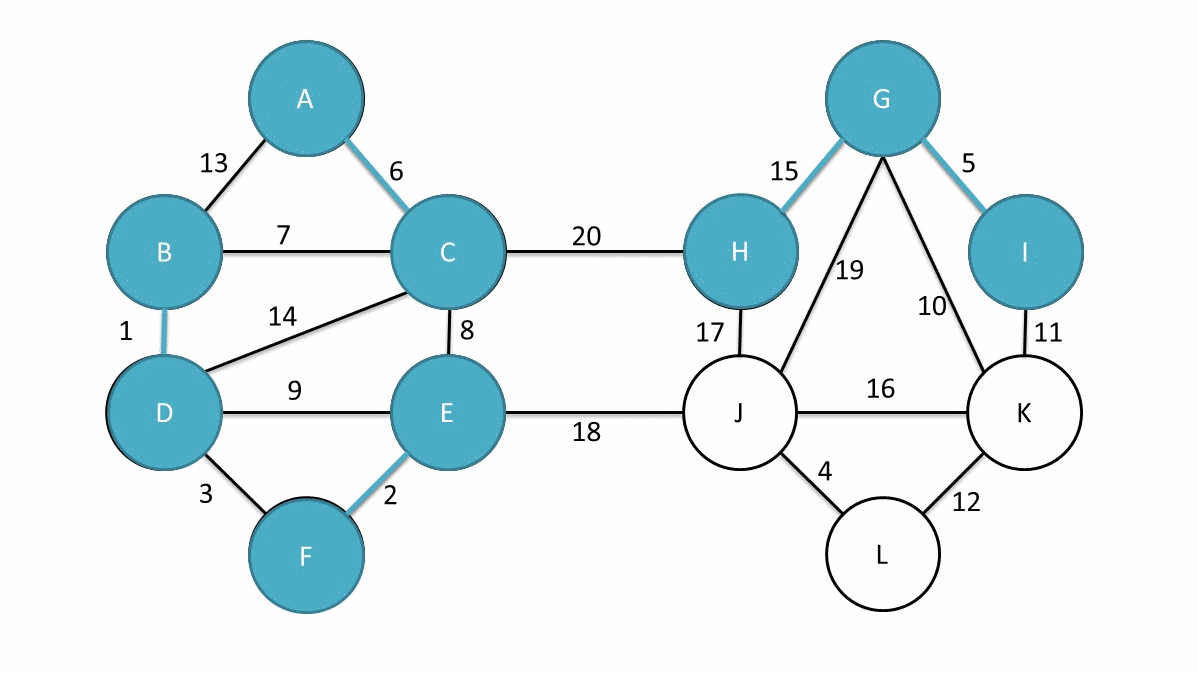
\includegraphics[width = 1\textwidth]{baruvka-example/frame_14_delay-2s.png}
\end{frame}
\begin{frame}
    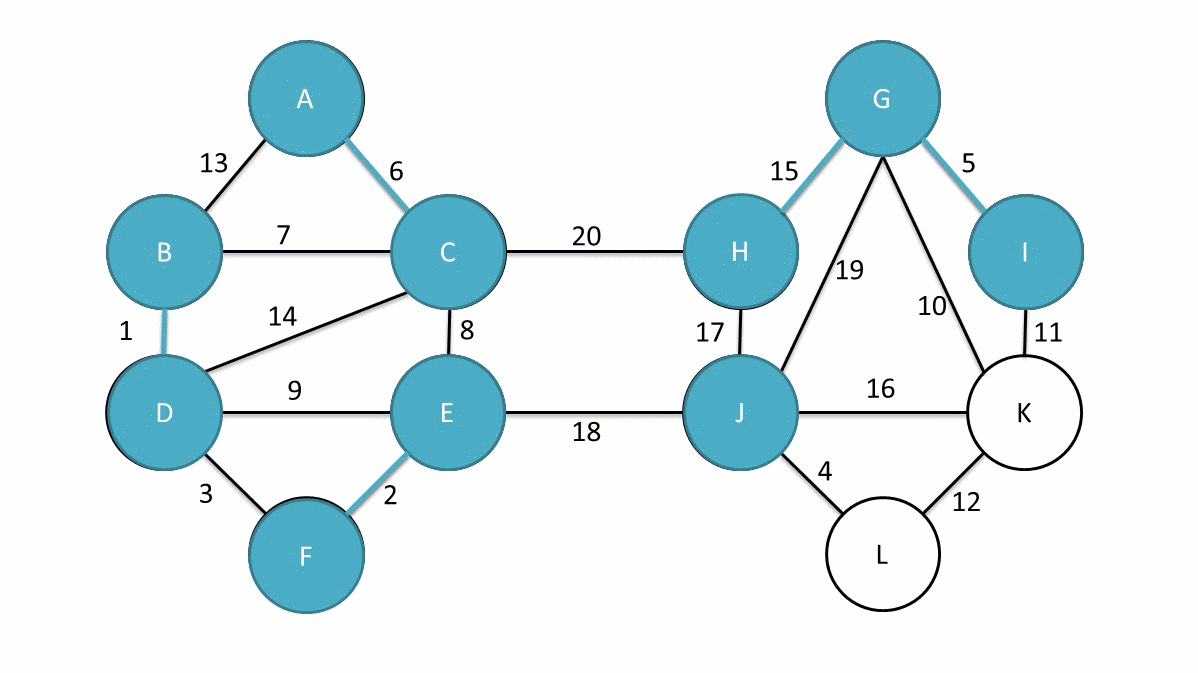
\includegraphics[width = 1\textwidth]{baruvka-example/frame_15_delay-1s.png}
\end{frame}
\begin{frame}
    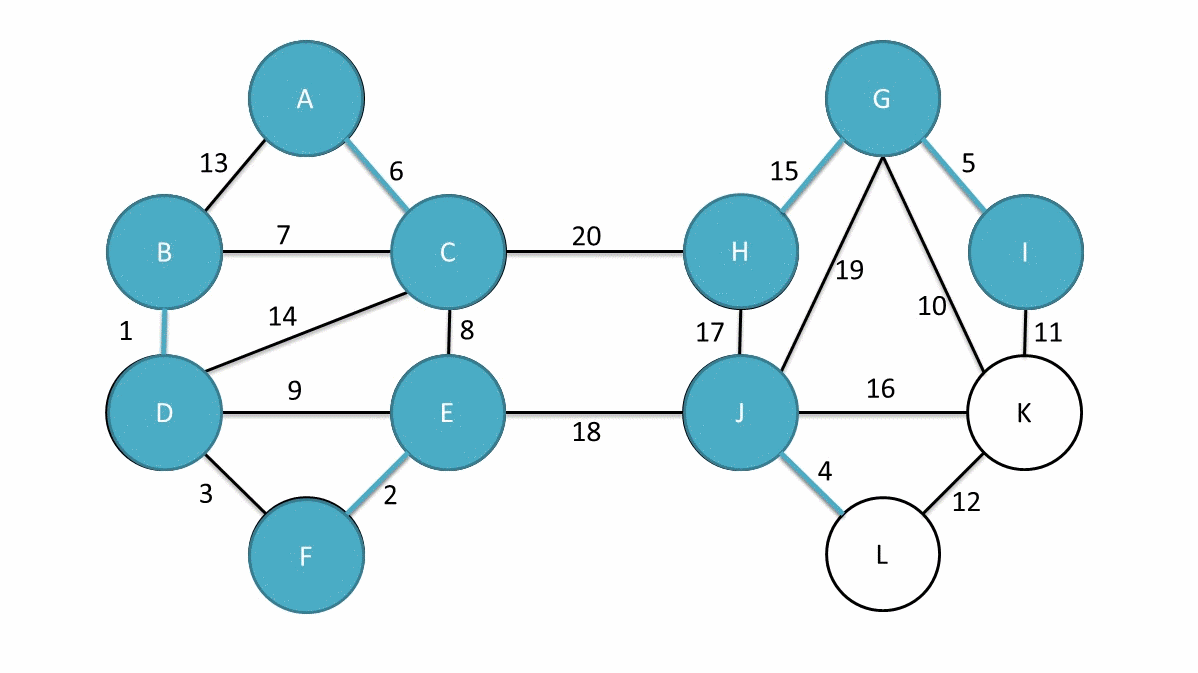
\includegraphics[width = 1\textwidth]{baruvka-example/frame_16_delay-1s.png}
\end{frame}
\begin{frame}
    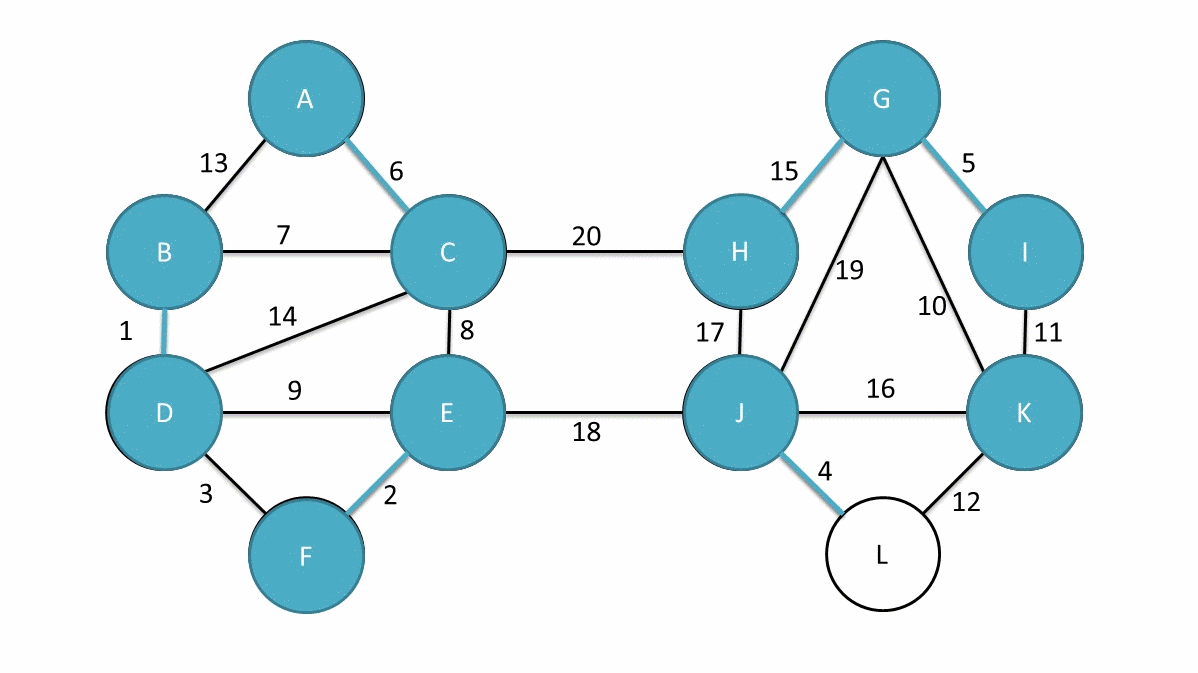
\includegraphics[width = 1\textwidth]{baruvka-example/frame_17_delay-1s.png}
\end{frame}
\begin{frame}
    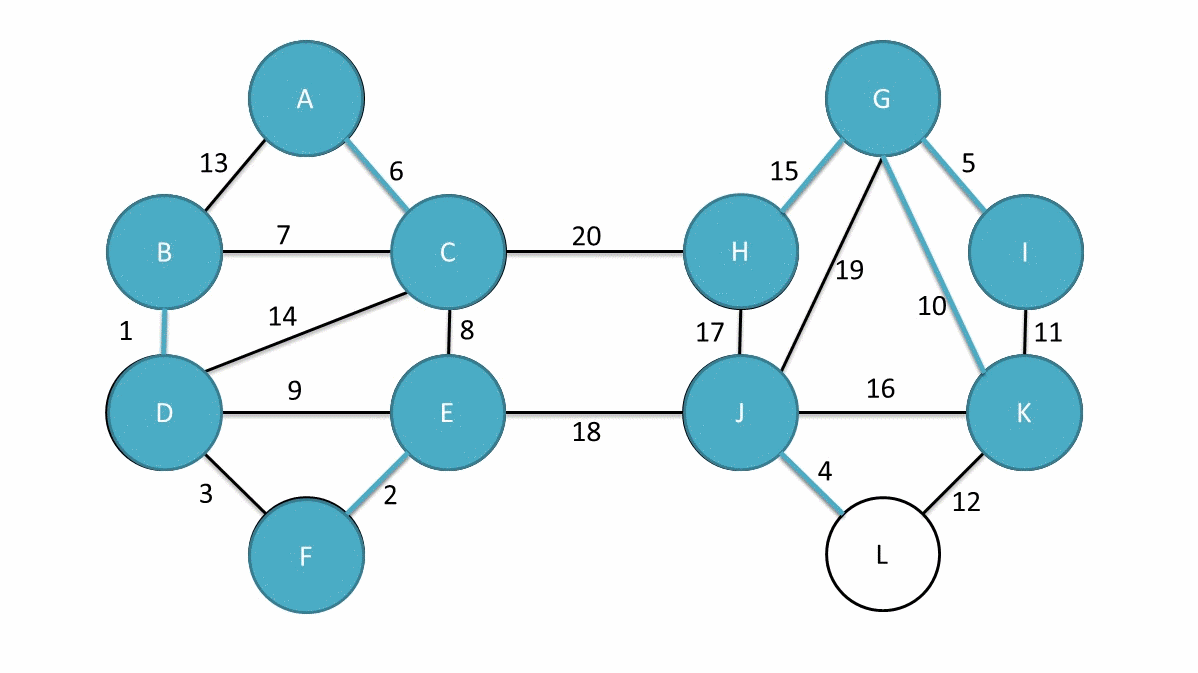
\includegraphics[width = 1\textwidth]{baruvka-example/frame_18_delay-1s.png}
\end{frame}
\begin{frame}
    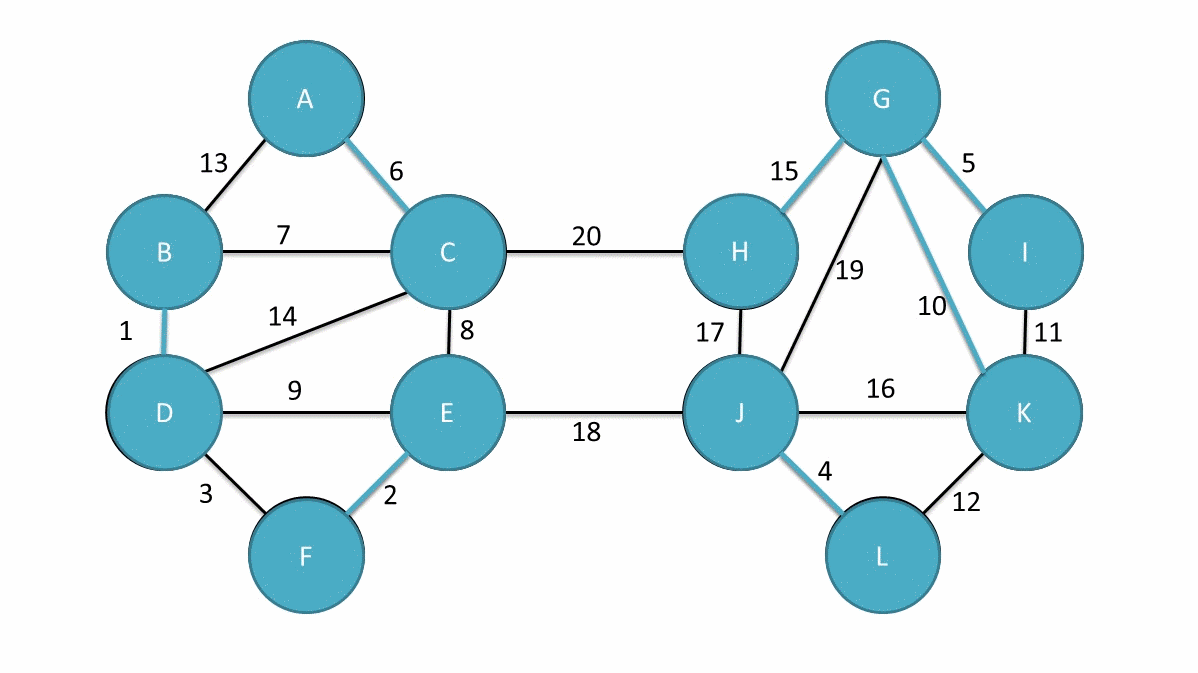
\includegraphics[width = 1\textwidth]{baruvka-example/frame_19_delay-2s.png}
\end{frame}
\begin{frame}
    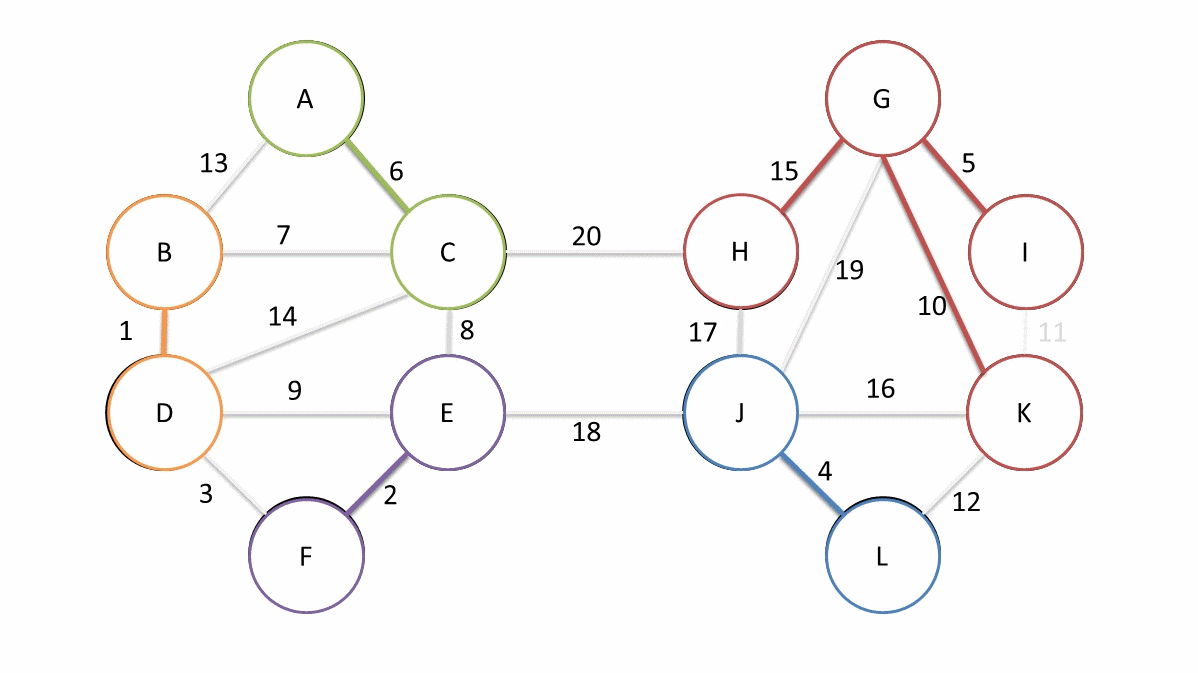
\includegraphics[width = 1\textwidth]{baruvka-example/frame_20_delay-3s.png}
\end{frame}
\begin{frame}
    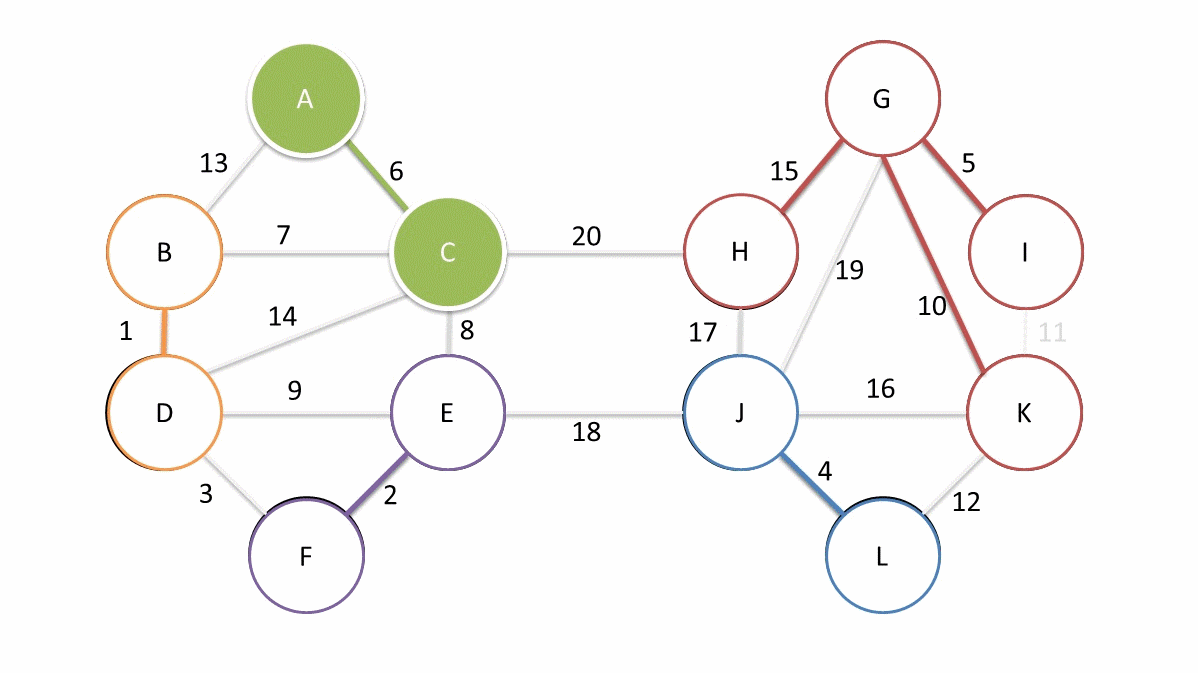
\includegraphics[width = 1\textwidth]{baruvka-example/frame_21_delay-1s.png}
\end{frame}
\begin{frame}
    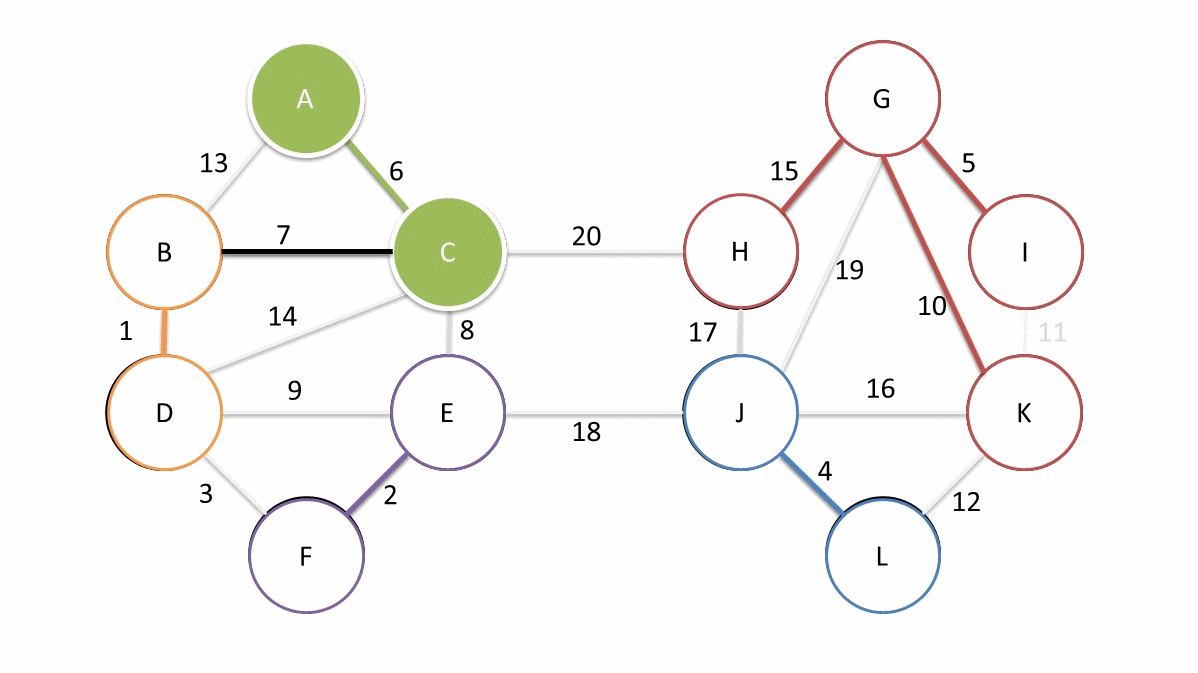
\includegraphics[width = 1\textwidth]{baruvka-example/frame_22_delay-1s.png}
\end{frame}
\begin{frame}
    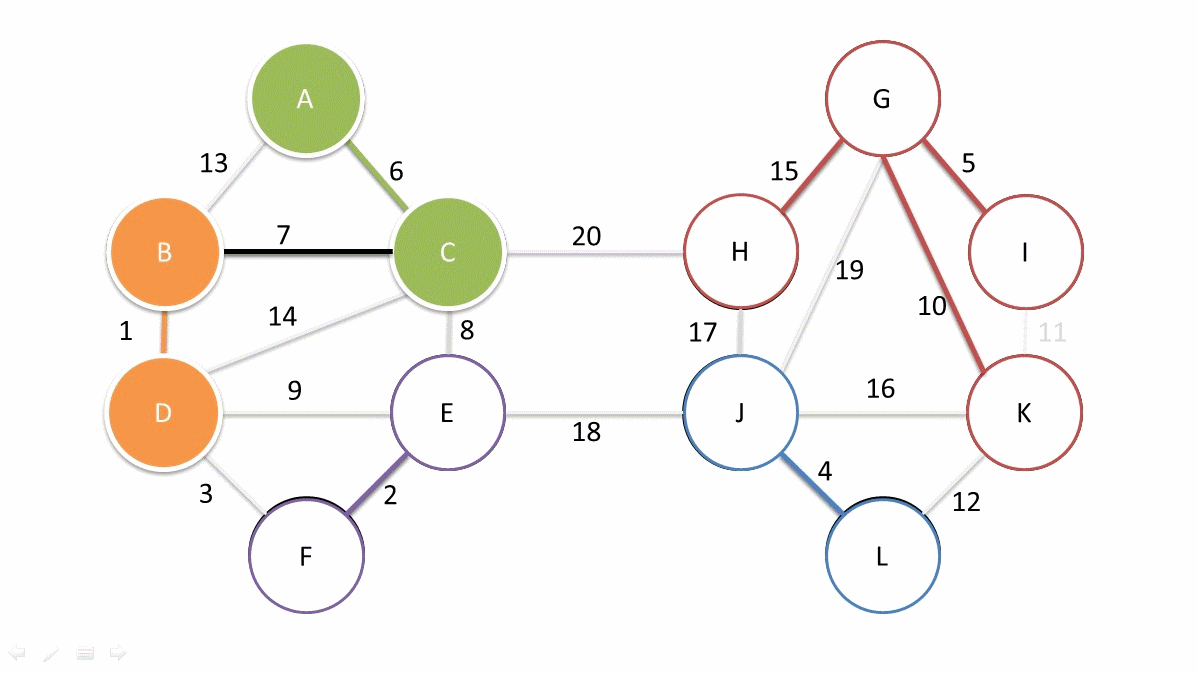
\includegraphics[width = 1\textwidth]{baruvka-example/frame_23_delay-1s.png}
\end{frame}
\begin{frame}
    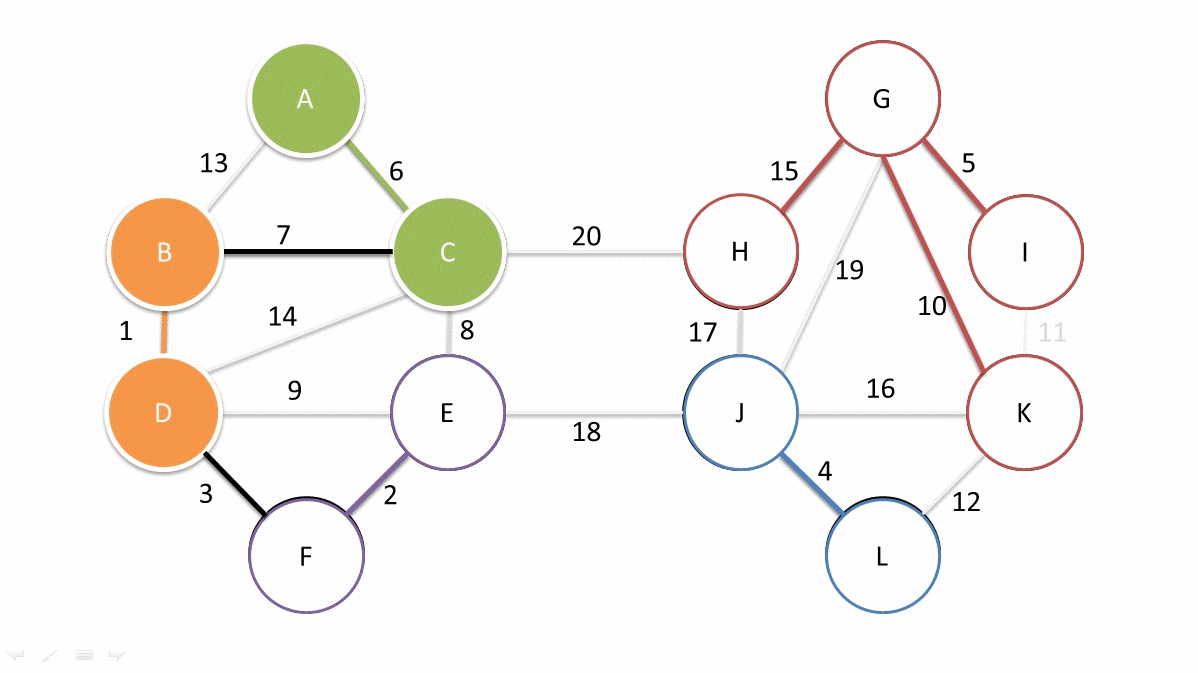
\includegraphics[width = 1\textwidth]{baruvka-example/frame_24_delay-1s.png}
\end{frame}
\begin{frame}
    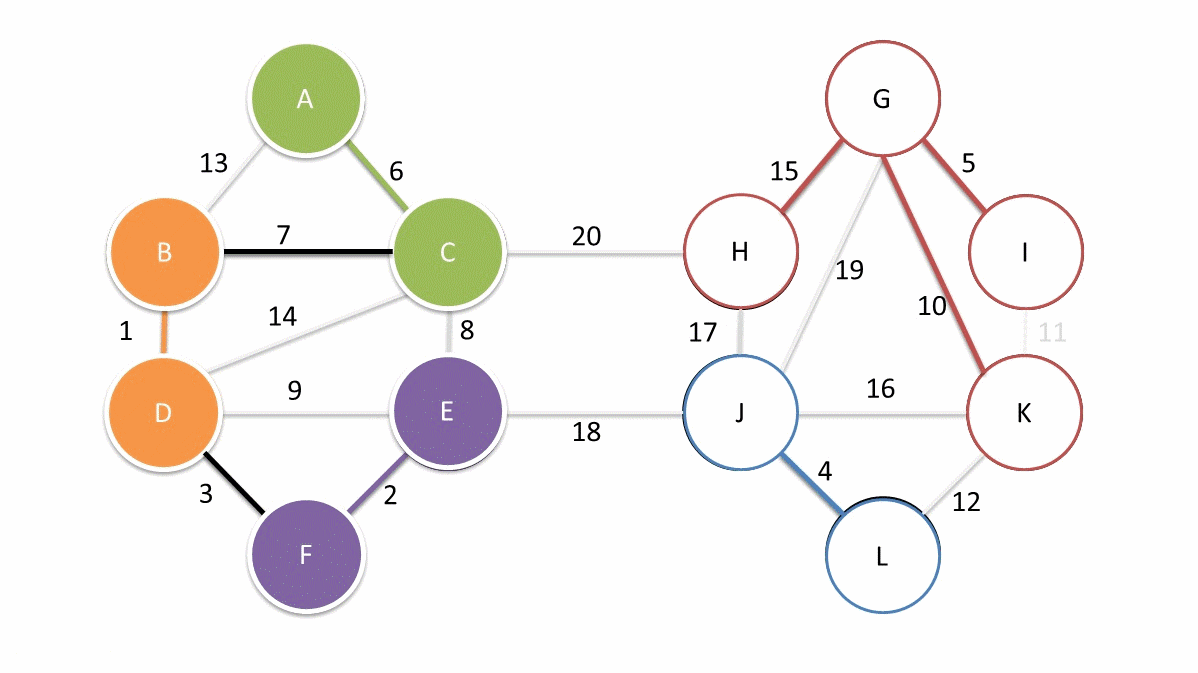
\includegraphics[width = 1\textwidth]{baruvka-example/frame_25_delay-2s.png}
\end{frame}
\begin{frame}
    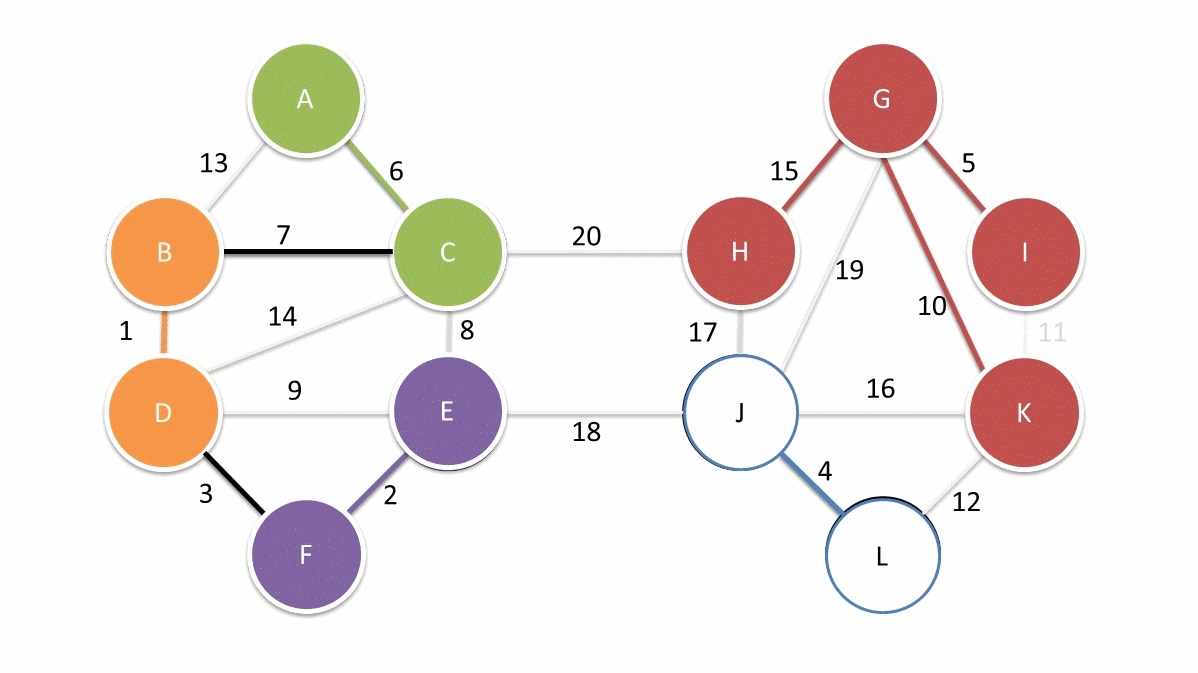
\includegraphics[width = 1\textwidth]{baruvka-example/frame_26_delay-1s.png}
\end{frame}
\begin{frame}
    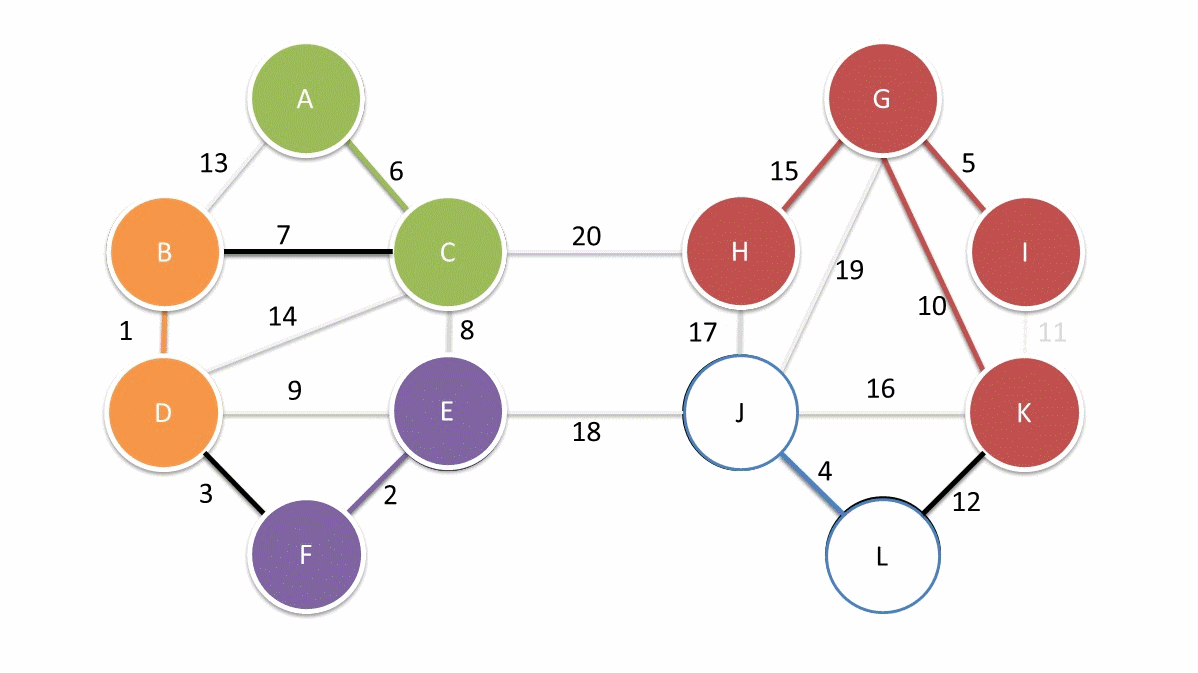
\includegraphics[width = 1\textwidth]{baruvka-example/frame_27_delay-1s.png}
\end{frame}
\begin{frame}
    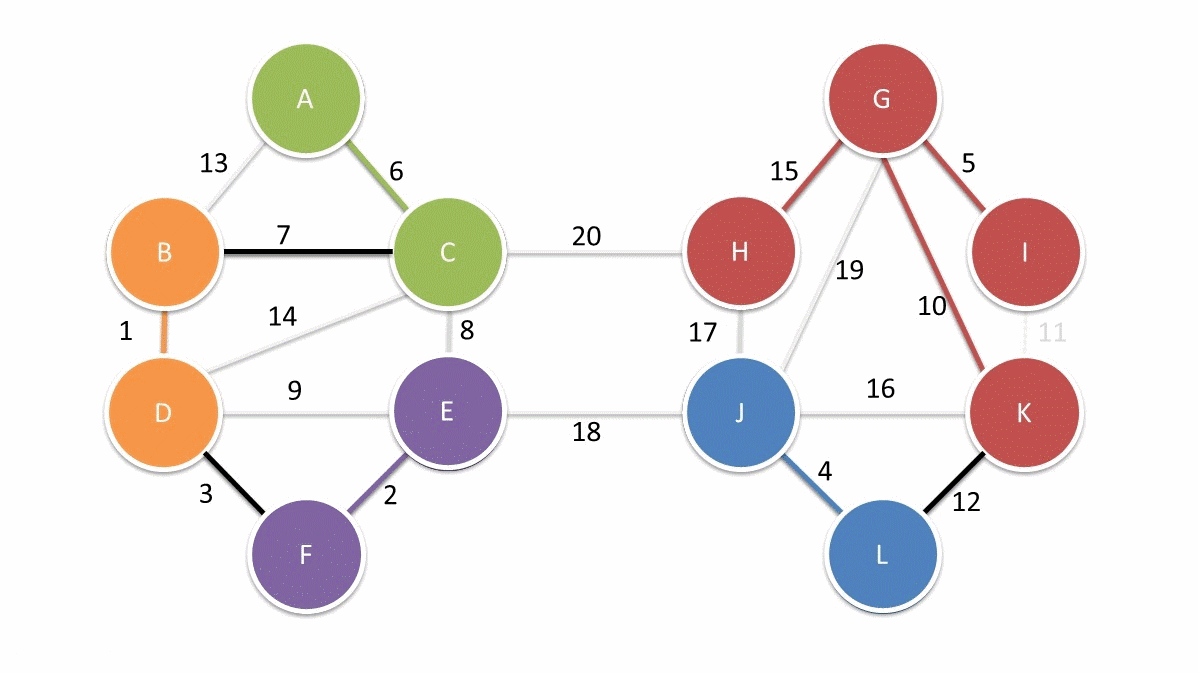
\includegraphics[width = 1\textwidth]{baruvka-example/frame_28_delay-2s.png}
\end{frame}
\begin{frame}
    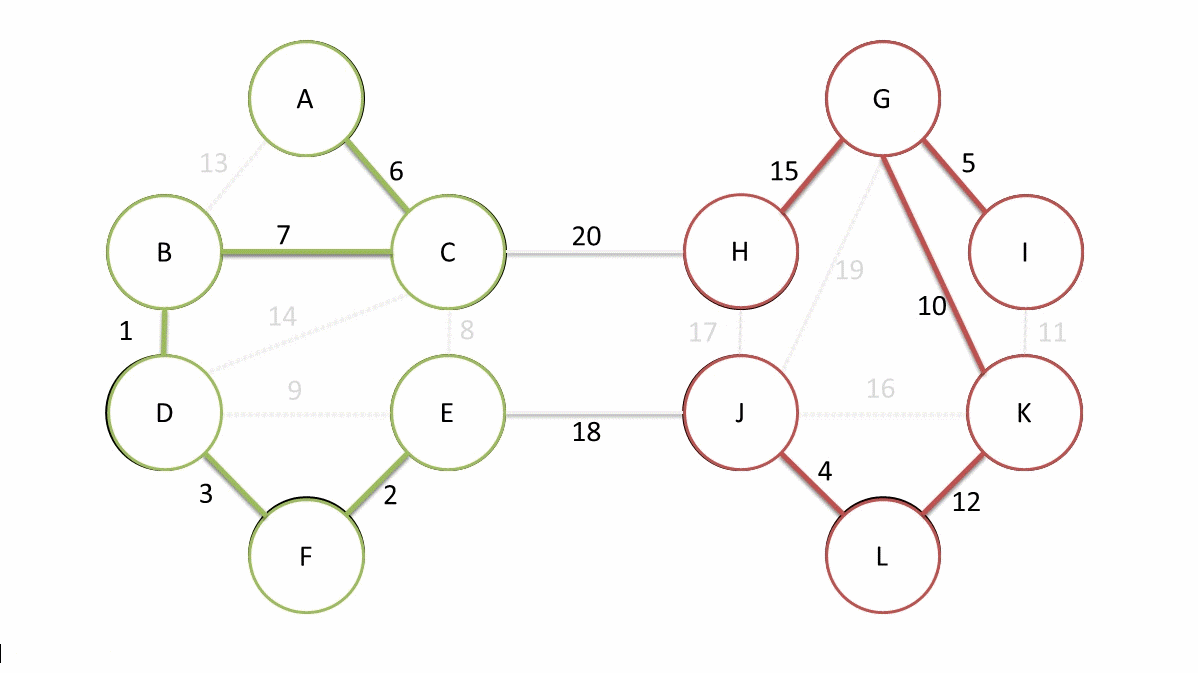
\includegraphics[width = 1\textwidth]{baruvka-example/frame_29_delay-3s.png}
\end{frame}
\begin{frame}
    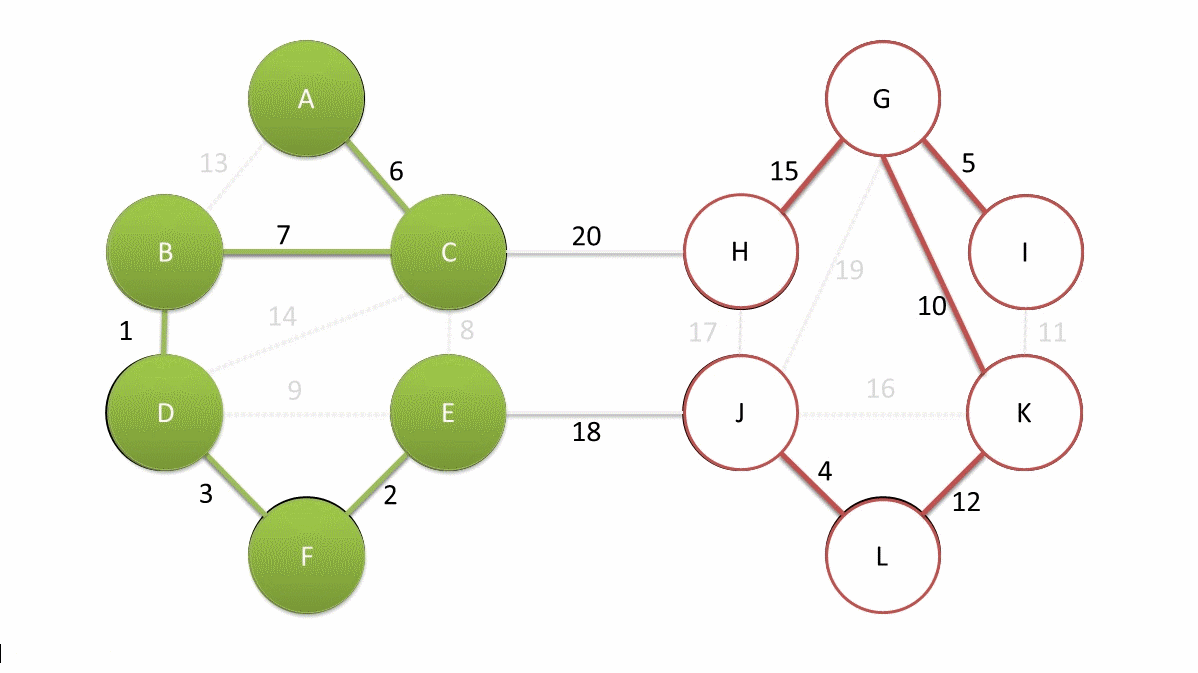
\includegraphics[width = 1\textwidth]{baruvka-example/frame_30_delay-1s.png}
\end{frame}
\begin{frame}
    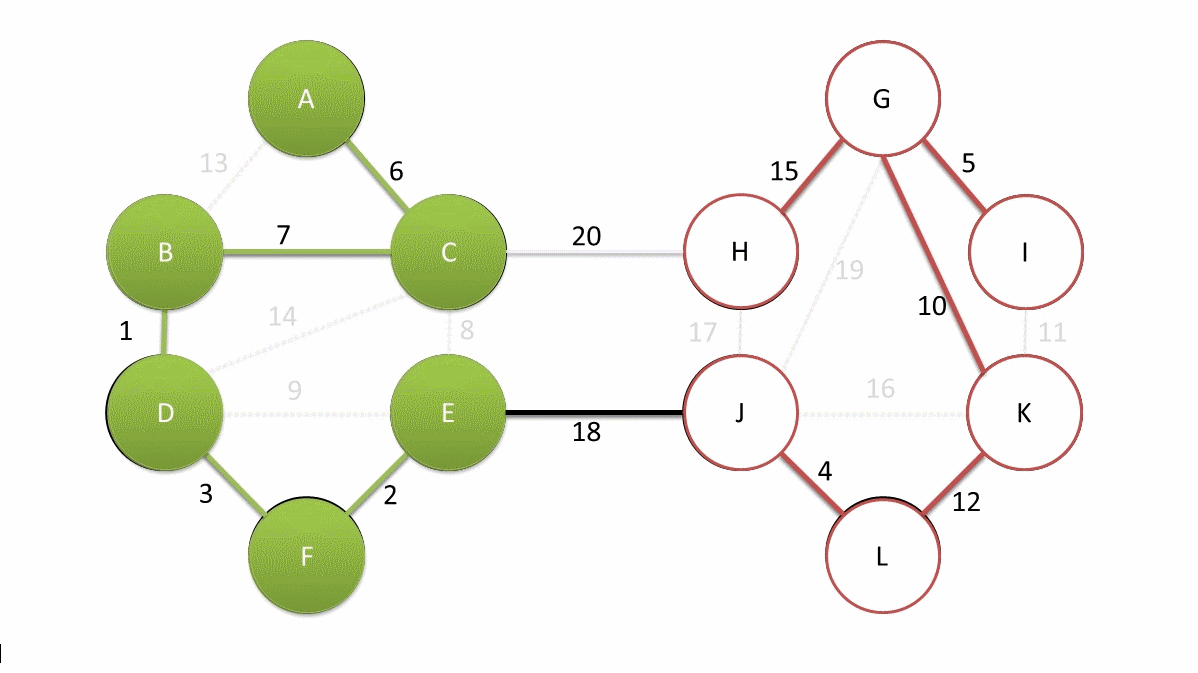
\includegraphics[width = 1\textwidth]{baruvka-example/frame_31_delay-1s.png}
\end{frame}
\begin{frame}
    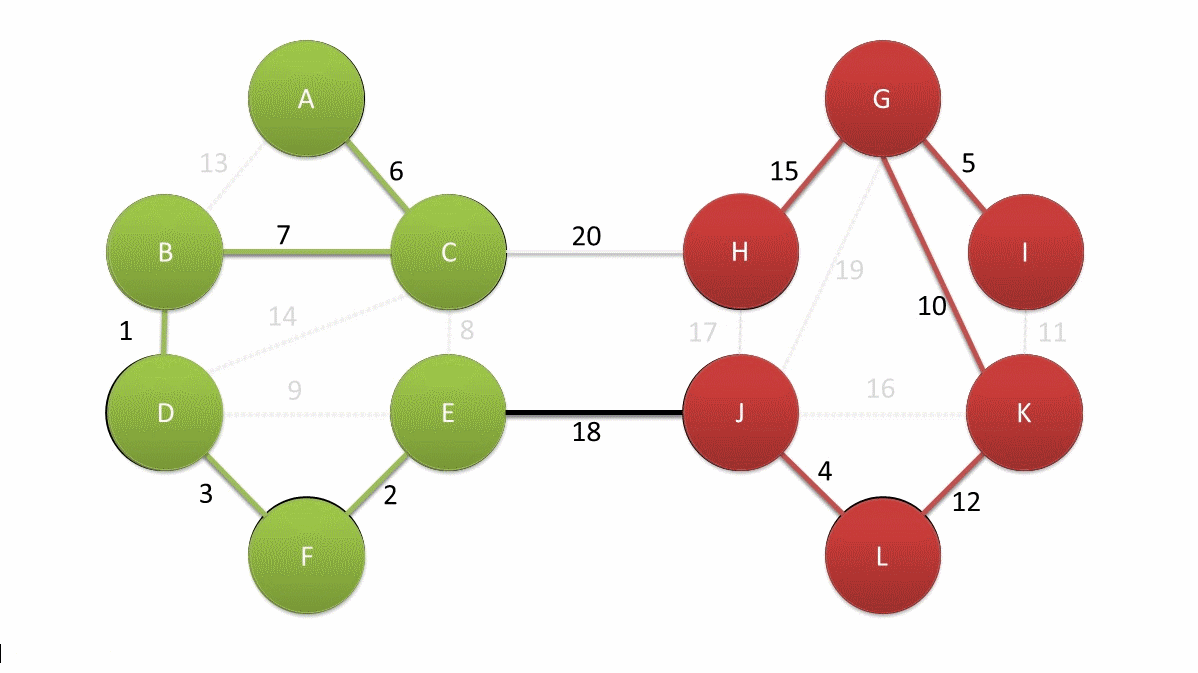
\includegraphics[width = 1\textwidth]{baruvka-example/frame_32_delay-2s.png}
\end{frame}
\begin{frame}
    And here is the final solution. The MST has a weight of 83 and the chosen edges are:
    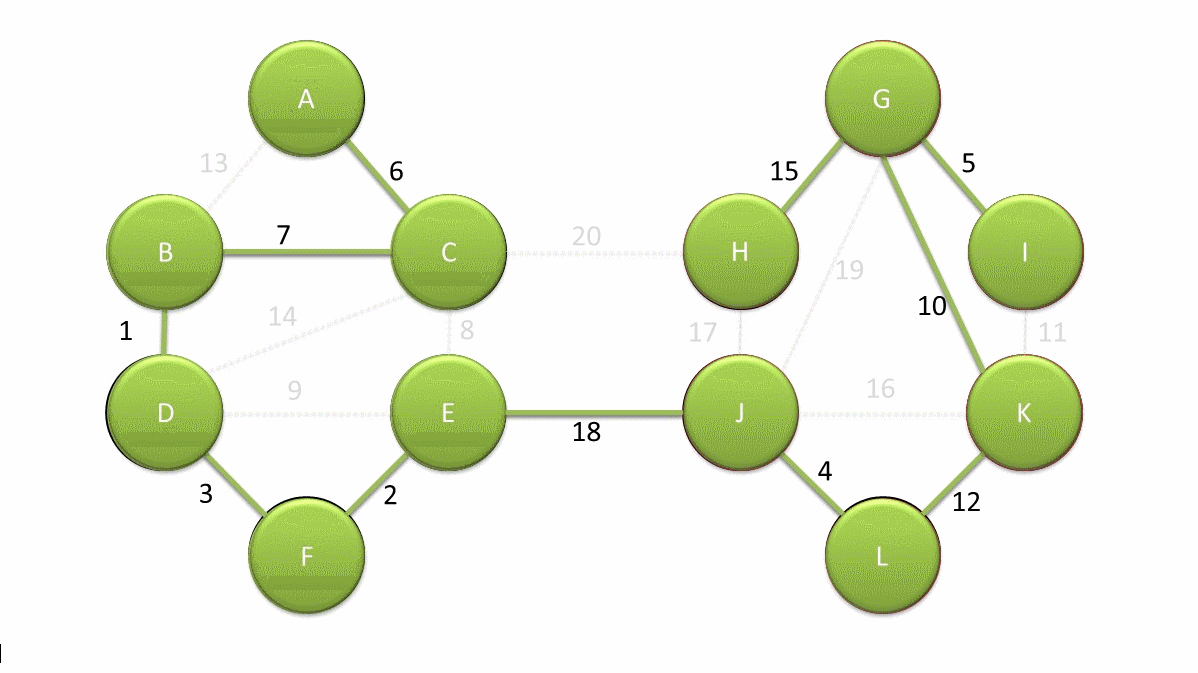
\includegraphics[width = 1\textwidth]{baruvka-example/frame_33_delay-4s.png}
\end{frame}

\section{Implementation}
\begin{frame}
    \tableofcontentscurrent
\end{frame}

\begin{frame}[fragile,shrink=4]
    \frametitle{Borůvka's Algorithm}
    \begin{semiverbatim}
        Input: A weighted undirected graph G = (V, E)
        Output: F, a minimum spanning forest of G
        
        Initialize a forest F to (V, E') where E' = {}
        
        completed := false
        while not completed do
            Find the connected components of F and assign to each vertex its component
            Initialize the cheapest edge for each component to "None"
            for each edge uv in E, where u and v are in different components of F:
                let wx be the cheapest edge for the component of u
                if is-preferred-over(uv, wx) then
                    Set uv as the cheapest edge for the component of u
                let yz be the cheapest edge for the component of v
                if is-preferred-over(uv, yz) then
                    Set uv as the cheapest edge for the component of v
            if all components have cheapest edge set to "None" then
                completed := true
            else
                completed := false
                for each component whose cheapest edge is not "None" do
                    Add its cheapest edge to E'

        function is-preferred-over(edge1, edge2) is
            return (edge2 is "None") or
                    (weight(edge1) < weight(edge2)) or
                    (weight(edge1) = weight(edge2) and tie-breaking-rule(edge1, edge2))
        
        function tie-breaking-rule(edge1, edge2) is
            The tie-breaking rule; returns true if and only if edge1
            is preferred over edge2 in the case of a tie.
    \end{semiverbatim}
\end{frame}

\section{Complexity Analysis}
\begin{frame}
    \tableofcontentscurrent
\end{frame}

\begin{frame}
    \begin{lemma}
        There would be at most $O(log \; V)$ steps of merging trees. 
    \end{lemma}
    \begin{lemma}
        Each step of merging trees, takes $O(V + E)$.
    \end{lemma}
    \begin{fact}
        The time complexity for Borůvka’s algorithm is $O((V + E) log \; V)$.
    \end{fact}

    \begin{fact}
        The memory usage for Borůvka’s algorithm is $O(V + E)$.
    \end{fact}
\end{frame}

\section{Correctness}
\begin{frame}
    \tableofcontentscurrent
\end{frame}

\begin{frame}
    \begin{lemma}
        The algorithm leads to a connected graph.
    \end{lemma}
    
    \begin{lemma}
        The algorithm leads to an acyclic graph.
    \end{lemma}
    
    \begin{fact}
        The algorithm leads to a tree with $V$ vertices.
    \end{fact}

    \begin{lemma}
        The algorithm gives the MST (Prove by induction. There always exists some MST containing these edges.).
    \end{lemma}
\end{frame}

\section{Other Algorithms}
\begin{frame}
    \tableofcontentscurrent
\end{frame}

\begin{frame}
    \begin{beamerboxesrounded}[shadow=true]{Other algorithms}
        Other algorithms for this problem include Prim's algorithm and Kruskal's algorithm.
    \end{beamerboxesrounded}

    \begin{fact}
        Prim algorithm can be done in $O(E + V log \; V)$ using complicated data structures like fibonacci heap.
    \end{fact}

    \begin{fact}
        Kruskal algorithm can be done in $O((V + E) log \; E)$ since it needs the sorted list of edges.
    \end{fact}
\end{frame}

\section{Applications}
\begin{frame}
    \tableofcontentscurrent
\end{frame}

\begin{frame}
    \begin{beamerboxesrounded}[shadow=true]{Application 1}
        Fast parallel algorithms can be obtained by combining Prim's algorithm with Borůvka's.
    \end{beamerboxesrounded}

    \begin{beamerboxesrounded}[shadow=true]{Application 2}
        A faster randomized minimum spanning tree algorithm based in part on Borůvka's algorithm due to Karger, 
        Klein, and Tarjan runs in expected $O(E)$ time.
    \end{beamerboxesrounded}

    \begin{beamerboxesrounded}[shadow=true]{Application 3}
        The best known (deterministic) minimum spanning tree algorithm by Bernard Chazelle is also based in part on 
        Borůvka's and runs in $O(E α(E,V))$ time, where $α$ is the inverse Ackermann function.
    \end{beamerboxesrounded}
    
    \begin{fact}
        These randomized and deterministic algorithms combine steps of Borůvka's algorithm, reducing the number of 
        components that remain to be connected, with steps of a different type that reduce the number of edges between 
        pairs of components.
    \end{fact}
\end{frame}

\begin{frame}
    \begin{figure}
        \centering
        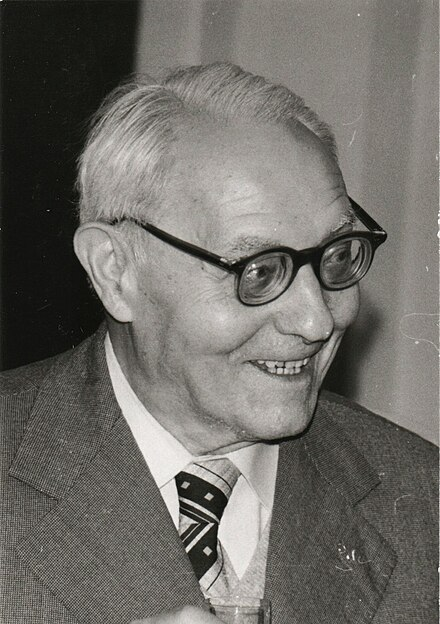
\includegraphics[width=0.45\textwidth]{images/Otakar_Boruvka.jpg}
        \caption{Otakar Borůvka}
    \end{figure}
\end{frame}

\section{References}
\begin{frame}
    \tableofcontentscurrent
\end{frame}

\begin{frame}{References}
    \bullet \url{en.wikipedia.org/wiki/Bor\%C5\%AFvka\%27s\_algorithm}

    \bullet \url{en.wikipedia.org/wiki/Otakar\_Bor\%C5\%AFvka}

    \bullet \url{cs.brown.edu/research/pubs/pdfs/1995/Karger-1995-RLT.pdf}

    \bullet \url{https://en.wikipedia.org/wiki/Prim\%27s\_algorithm}

    \bullet \url{https://en.wikipedia.org/wiki/Kruskal\%27s\_algorithm}
\end{frame}

\begin{frame}
    \frametitle{The End}
    \begin{center}
        \textbf{\huge{\emph{Thank You For Your Attention!}}}  
    \end{center}
\end{frame}

\end{document}